\documentclass[]{book}
\usepackage{longtable,booktabs}

\usepackage{amsthm}
\usepackage{amsmath}
%\usepackage{tipa}
%\usepackage{amssymb} %for some symbols
%\usepackage[]{fontspec}
\usepackage{titling}
\usepackage{emptypage}
\usepackage{titlesec, blindtext, color}
\definecolor{gray75}{gray}{0.75}
\newcommand{\hsp}{\hspace{20pt}}
\usepackage{polyglossia}
\usepackage[]{babel}
\setdefaultlanguage[]{spanish}


% +---------------+
% |   Cormorant   |
% +---------------+

\usepackage[T1]{fontenc}
%\newcommand{\fuenteprincipal}{Cormorant}
\setmainfont[Path = fonts/, BoldFont={Cormorant-bold.ttf}, ItalicFont={Cormorant-italic.ttf},]{Cormorant-Regular.ttf}
%\setromanfont{Cormorant}
%\newfontfamily\headingfont[]{Cormorant}


\usepackage{setspace} %for line spacing
\usepackage{fancyhdr}

\makeatletter
\newcommand\mycustomhead{%
   \@startsection{section}{1}{\z@}%
   {-3.5ex \@plus -1ex \@minus -.2ex}%
   {2.3ex \@plus.2ex}%
   {\normalfont\normalsize\bfseries}}
\newcommand\myhead[1]{\mycustomhead*{#1}}
\makeatother

% +-----------------+
% |  Article title  |
% +-----------------+

\titleformat{\chapter}[display] % only removes chapter number from first page, not heading
{\normalfont\huge\bfseries\centering}{}{20pt}{\Huge}

\newcommand{\autor}[1]{            % command to display the author name in a fancy way :)
  \begin{center}                   % center text
    \vspace*{-3.5em}               % reduce the amount of space on top of the name
    \textbf{\textit{\large #1}}    % display text in bold and italics
    \vspace*{+4em}                 % add some space after the name
  \end{center}
}


\onehalfspace

\clubpenalty=10000
\widowpenalty=10000


% +------------------------------+
% |   Per chapter bibliography   |
% +------------------------------+

% \usepackage{biblatex}
\usepackage[backend=biber,style=apa,language=spanish]{biblatex}
\usepackage{csquotes}
\DeclareLanguageMapping{spanish}{spanish-apa}
\addbibresource{bibliografia-No1.bib}



\usepackage[inner=4cm,top=3cm,outer=2.8cm, bottom=3cm]{geometry}
\usepackage[unicode=true]{hyperref}
\hypersetup{
            pdfborder={0 0 0},
            breaklinks=true}
\urlstyle{same}  % don't use monospace font for urls
% Fix footnotes in tables (requires footnote package)
\usepackage{graphicx,grffile}
\makeatletter
\def\maxwidth{\ifdim\Gin@nat@width>\linewidth\linewidth\else\Gin@nat@width\fi}
\def\maxheight{\ifdim\Gin@nat@height>\textheight\textheight\else\Gin@nat@height\fi}
\makeatother
% Scale images if necessary, so that they will not overflow the page
% margins by default, and it is still possible to overwrite the defaults
% using explicit options in \includegraphics[width, height, ...]{}
\setkeys{Gin}{width=\maxwidth,height=\maxheight,keepaspectratio}
\IfFileExists{parskip.sty}{%
\usepackage{parskip}
}{% else
\setlength{\parindent}{0pt}
\setlength{\parskip}{6pt plus 2pt minus 1pt}
}
\setlength{\emergencystretch}{3em}  % prevent overfull lines
\providecommand{\tightlist}{%
  \setlength{\itemsep}{0pt}\setlength{\parskip}{0pt}}
\setcounter{secnumdepth}{0}
% Redefines (sub)paragraphs to behave more like sections
\ifx\paragraph\undefined\else
\let\oldparagraph\paragraph
\renewcommand{\paragraph}[1]{\oldparagraph{#1}\mbox{}}
\fi
\ifx\subparagraph\undefined\else
\let\oldsubparagraph\subparagraph
\renewcommand{\subparagraph}[1]{\oldsubparagraph{#1}\mbox{}}
\fi

% set default figure placement to htbp
\makeatletter
\def\fps@figure{htbp}
\makeatother
\setlength{\parindent}{2em} 


\fancyhead{} % clear all header fields
\fancyfoot{} % clear all footer fields
\fancyhead[C]{ \footnotesize Diáphora - Número 1} 
\fancyfoot[C]{\small \thepage}
%Ahora sólo falta decidir qué se quiere en los encabezados.


\begin{document}
\pagestyle{fancy}
	
\title{Diáphora}
\author{Revista de Estudiantes de Filosofía de la Universidad de la
Sabana}

\maketitle


\textbf{Número 1}



\begin{longtable}[]{@{}ll@{}}
\toprule
\midrule
\endhead
Rector & Obdulio Velásquez Posada\tabularnewline
&\tabularnewline
Decano Facultad de Filosofía y Ciencias Humanas & Bogdan
Piotrowski\tabularnewline
&\tabularnewline
Directora del Programa de Filosofía & Carmen Elena
Arboleda\tabularnewline
&\tabularnewline
Representante de Estudiantes & María Camila Sarmiento
Oviedo\tabularnewline
&\tabularnewline
Comité Editorial & Martín Buenahora \tabularnewline
& Pablo Rivas Robledo\tabularnewline
& Juan Camilo Espejo Serna\tabularnewline
& Daniel Esteban García Saavedra\tabularnewline
& José Miguel Rueda Vásquez\tabularnewline
\bottomrule
\end{longtable}

\noindent Semestre 2018-1. Número 1.

\noindent Diáphora es una revista de publicación académica con frecuencia
semestral, editada por estudiantes de filosofía.

\noindent Contacto: \href{mailto:diaphora@unisabana.edu.co}{\nolinkurl{diaphora@unisabana.edu.co}}



El material creado para esta publicación puede ser distribuido, copiado
y exhibido por teceros si se muestra en los créditos. No se puede
obtener ningún beneficio comercial y las obras derivadas tienen que
estar bajo los mismos términos de licencia que el trabajo original.

Los textos presentados aquí expresan la opinión de sus respectivos
autores y la Universidad de La Sabana no se compromete directamente con
la opinión que expresan.

Diáphora desea agradecer a todas las personas que colaboraron de una u
otro manera en la realización de este número. Ellos saben quiénes son,
les estamos inmensamente agradecidos.
\begin{center}

\includegraphics[width=2.24419in,height=0.78333in]{media/image1.png}
\end{center}

\tableofcontents

\chapter{\texorpdfstring{\textbf{Carta del
editor}}{Carta del editor}}\label{carta-del-editor}

Es el esfuerzo de muchos estudiantes de pregrado de Filosofía de la
Universidad de La Sabana lo que permite que estas páginas lleguen a ojos
distintos. Desconozco en gran parte el proceso antes de que llegara a
mis manos, por lo que me veo obligado a contarlo desde mi perspectiva. A
los que vinieron antes de nosotros les estamos inmensamente agradecidos.

En mi primer semestre en la carrera de Filosofía (enero-mayo de 2015)
tuve la fortuna de cursar la materia Lectura y Escritura de Textos
Filosóficos con la profesora Milena Patiño, quien, al final del
semestre, nos invitó a buscar espacios editoriales para la publicación
de nuestros futuros trabajos. La idea entusiasmó a muchos. Para finales
de 2016 no sólo estábamos pensando en publicar varios trabajos,
estábamos convencidos que incluso mejor que publicar nuestros textos
externamente sería crear nuestro propio espacio de difusión. La idea nos
entusiasmó aún más. Durante diversas reuniones con el Dr. Bogdan
Piotrowski, Decano de la Facultad de Filosofía, y con otros estudiantes
definimos, con bombos y platillos, pautas de publicación, consejos
editoriales, comités gráficos e incluso el nombre de la
revista\footnote{En un primer momento el nombre escogido fue Agón, una
  explicación etimológica proporcionada por el profesor Ronald Forero
  nos convenció que no era el nombre que en realidad buscábamos.
  Diáphora tiene dos significados, diferencia y repetición. Se eligió
  este nombre porque en últimas la labor filosófica es repetitiva,
  escribir es repetir ideas, presentar un texto es volver a leerlo,
  revisar un texto es volver a escribirlo, publicarlo es que el lector
  repita en su cabeza las ideas del autor. Queremos que este proceso se
  repita en nuestra revista y hacerlo de la mejor manera para así marcar
  la diferencia.}. Teníamos todos menos los textos para publicar, y esta
situación, además de ser preocupante, no cambiaba.

Un problema adicional surgió semanas después, cuando un grupo de
estudiantes, representando a la revista, se reunió con la Dirección de
Publicaciones. Esta dependencia les anunció que, para lograr cualquier
apoyo por parte de la universidad, por lo menos debíamos tener
asegurados tres números de la revista. Para tener fondos para la revista
necesitábamos una producción académica constante, pero no teníamos si
quiera textos confirmados para una primera edición. Por lo tanto, la
posibilidad de hacer una revista estudiantes totalmente avalada por la
Facultad y por la Universidad se esfumaba e íbamos perdiendo el
entusiasmo.

Esta situación cambió en el segundo semestre de 2017. Para entonces, el
profesor Juan Camilo Espejo-Serna comenzó a dictar la materia
\emph{Metodología de la Investigación Filosófica,} cuyo trabajo final
consiste en que cada estudiante presente un proyecto de tesis. Para la
socialización de los proyectos, el profesor Juan Camilo juntó dos
proyectos que quería consolidar: (1) un semillero de investigación y (2)
un foro interno. Al mismo tiempo, Juan Camilo, quien no era parte de la
planta profesoral de la universidad cuando propusimos la revista por
primera vez, me propuso crear una versión preliminar de la revista y que
poco a poco fuéramos cumpliendo los requisitos exigidos para después
consolidar la revista.

Conectar los proyectos de Juan Camilo con su propuesta fue clave para la
consolidación de Diáphora. Se crearía un foro interno para para
presentar los trabajos finales de \emph{Metodología} y otros productos
académicos; sería un evento auspiciado y organizado por el semillero; y
los textos presentados serían la fuente principal de productos
publicables en la revista. De esta manera solucionábamos el problema
inicial y asegurábamos continuidad de la revista.

El I Foro interno del semillero de investigación en Ciencia, Lógica y
Metafísica (Krínein) se realizó el 3 de noviembre en el salón A-209 de
la Universidad de La Sabana de 1:00 PM a 6:00 PM y contó con la
participación como ponentes de 7 estudiantes de la Facultad y un
graduado de esta. La programación fue la siguiente:

\begin{table}[]
	\centering
	\begin{tabular}{@{}lcl@{}}
		\toprule
		\textbf{Nombre}                    & \textbf{Horario}        & \textbf{Título de la ponencia} \\ \midrule
		Cristian Felipe González Hernández & \textbf{13:00 - 13:30}  & Relativismo y realismo ¿por qué aceptamos una \\ & &  ontología?                                             \\
		Paula Andrea Sierra Musse          & \textbf{13:30 - 14:00}  & ¿Es la ley necesariamente vaga?                                                                      \\
		Pablo Rivas Robledo                & \textbf{14:00 -  14:30} & Una solución a la paradoja de la reforma de los  \\ & &   mecanismos de reforma de las normas constitucionales \\
		Descanso                           & \textbf{14:30 - 14:45}  &                                                                                                      \\
		Lina Margarita Gómez Ávila         & \textbf{14:45 - 15:15}  & La música es una experiencia humana no reductible  \\ & &  a propiedades físicas                              \\
		Juan Manuel Gaitán Sánchez         & \textbf{14:15 - 14:45}  & Criterios de identidad-tipo de las experiencias:  \\ & &  Qualia vs. Objetos intencionales                    \\
		Descanso                           & \textbf{15:45 - 16:00}  &                                                                                                      \\
		Tatiana Gómez Sánchez              & \textbf{16:00 -  16:30} & ¿Es posible escuchar de nuevo y en vivo una misma \\ & & improvisación musical?                             \\
		Miguel Ángel Prieto Castellanos    & \textbf{16:30 - 17:00}  & ¿Saber un lenguaje consiste en tener ciertas  \\ & &  representaciones mentales?                              \\
		Descanso                           & \textbf{17:00 - 17:15}  &                                                                                                      \\
		Juan Sebastián Cáceres             & \textbf{17:15 - 17:45}  & ¿Es la emergencia una alternativa válida y sustentable  \\ & &  al reduccionismo?                             \\ \bottomrule
	\end{tabular}
\end{table}

El evento fue moderado por el profesor Juan Camilo y contó con la
participación de estudiantes y profesores de la Facultad. Así mismo, el
profesor John Anderson Pinzón Duarte y la profesora María Elvira Acuña
se encararon de formular preguntas al final de cada
intervención\footnote{Aprovecho este espacio para agradecer al profesor
  Ángel Rivera de la Universidad San Buenaventura, quien nos ayudó
  contactando parte del Comité Editorial.}. Todos les estamos
inmensamente agradecidos a los asistentes y de igual manera agradecemos
los Chocorramos y la gaseosa proporcionada por el profesor Juan Camilo
durante los descansos.

\begin{flushright}
	Pablo Rivas Robledo

Chía, 13 de marzo de 2018
\end{flushright}

\chapter{\texorpdfstring{\textbf{Presentación de los
textos}}{Presentación de los textos}}\label{presentaciuxf3n-de-los-textos.}

Los textos que componen este volumen se presentan en el mismo orden que
fueron sustentados el 3 de noviembre de 2017. A continuación, se
presenta un breve resumen lo que fue cada presentación. El primer texto
está a cargo de Cristian Felipe González, quien, compara dos sistemas
ontológicos, el esencialista y el relativista, intentando explicar qué
hace que una ontología tenga mayor fuerza explicativa que otra. Del
primero, afirma el ponente, Aristóteles y Putnam son los principales
defensores, mientras que Quine presenta una ontología relativista. Los
criterios que presenta son (1) la sencillez teórica, que maximiza el
poder explicativo; y (2) toda ontología debe (2.1) responder si es
posible sostener un conocimiento cierto sobre el mundo y (2.2) debe
establecer un saber que se resista a preguntas escépticas.

El producto de Paula Sierra es un valioso aporte al análisis filosófico
del lenguaje en el Derecho. En su trabajo \emph{¿Es la ley necesarimente
vaga}? Sierra parte de los argumentos de Russell sobre la vaguedad del
lenguaje para demostrar que en tanto el lenguaje natural es
necesariamente vago, y siendo el Derecho un producto de los lenguajes
naturales, la ley es necesariamente vaga. Como bien dice la autora, eso
puede ser perjudicial, sin embargo, Sierra demuestra que en ciertas
ocasiones se necesita que la ley sea vaga para garantizar un nivel de
efectividad jurídica. Sin este carácter, afirma la autora existiría una
problemática en la aplicación de muchas normas.

Pablo Rivas Robledo presenta un escrito en el cual se propone una
solución a la paradoja de la auto-modificación. Esta paradoja surge en
tanto en sistemas de reglas cuyas reglas son modificables, al parecer no
existe una regla que permita modificar la regla que autoriza la
modificación, creación o eliminación de cualquier otra regla del sistema
(regla de competencia). De ser esto cierto, en tanto no hay una regla
que autorice la modificación de la regla de competencia, la regla de
competencia no sería parte del sistema. Pero dado que la regla de
competencia sí hace parte del sistema, entonces no se puede aceptar la
conclusión anterior. La solución planteada es que puede haber una
modificación válida de la regla de competencia por el mismo
procedimiento que esta establece, a pesar de problemas de
autorreferencia parcial. Por obvias razones, recomiendo especialmente la
lectura de este trabajo.

Margarita Gómez presenta una interesante y novedosa crítica a uno de los
proyectos filosóficos más importantes del siglo XX. Identificando el
fisicalismo como la postura que sostiene que la persona y todos sus
atributos psicológicos no son nada más que su cuerpo y todas sus
propiedades físicas, Gómez propone la experiencia artística como un
fenómeno que, a pesar de caracterizar al ser humano, no es reducible a
fenómenos físicos. Para probarlo, la ponente modifica el experimento
mental de \emph{El cuarto de María} (Mary's room) para poner María, la
super-científica, en un cuarto con una partitura, pero sin la capacidad
de escucharla. La autora argumenta que a pesar de Mary conoce las
propiedades físicas de la partitura, cuando la escucha por primera vez
se enfrenta con una experiencia que no podía ser explicada en los
términos físicos con los que disponía anteriormente. En tanto la
experiencia artística es de esta índole, concluye la autora, el
fisicalismo no puede explicar este tipo de experiencias.

La revista continua con el trabajo \emph{Criterios de identidad-tipo de
las experiencias: Qualia vs. Objetos intensionales}, presentado por Juan
Manuel Gaitán. En este trabajo, el autor se planteaba el siguiente
dilema: Tengo dos criterios para identificar las experiencias, es decir,
que determinan las experiencias, pero son mutuamente excluyentes, cuál
de estos identifica mejor la experiencia. Por un lado, están los qualia,
por el otro, los objetos intensionales. Los qualia, afirma el autor,
tienen una desventaja, son sólo algunas de varias propiedades del
objeto, y además no hay buenas razones para explicar la experiencia de
un objeto en términos de sólo algunas de las propiedades del objet. De
esta manera, Gaitán prefiere los objetos intensionales, en la medida que
gracias a estos se pueden identificar las diferentes experiencias
funcionalmente, superando así la limitación de que tenían los qualia.

La ponencia que presenta Tatiana Gómez fue la más polémica en el momento
de su presentación y espero que también al momento de su lectura. Su
trabajo comienza con la siguiente pregunta: ¿puedo escuchar de nuevo y
en vivo una misma improvisación musical? Para responderla, la autora
caracteriza la improvisación musical como una actividad espontánea,
efímera, irrepetible, incorregible y libre en la cual se hace música.
Con base a esto, usa la distinción tipo/caso en la ontología musical y
el concepto de \emph{performance} para responder a la pregunta. Según la
autora, hay un sentido en el que sí se puede escuchar de nuevo y en vivo
una misma improvisación, en tanto se conciba la improvisación como una
obra de su repetición por medio de un performance, en tanto se repite,
se tiene que el performance es la \emph{misma} obra. Sin embargo, es
imposible que coincidan espacio-temporalmente dos repeticiones de la
misma improvisación, por lo que no se podría escuchar la \emph{misma}
improvisación más de una vez.

El trabajo \emph{¿Saber un lenguaje consiste en tener ciertas
representaciones mentales}? presentado por Miguel Ángel Prieto
Castellanos se publica bajo el título \emph{Tengo en mente lo que usted
tiene en mente}, las razones del cambio de título las tiene en mente
sólo el autor. En este trabajo, se examina el papel que tienen las
representaciones mentales en las interacciones lingüísticas del día a
día. Prieto arguye que a pesar de que no necesitemos apelar a ninguna
entidad representacional para entender el significado de las oraciones
en un primer momento, la introducción de prácticas lingüísticas más
complejas como las implicaturas o las metáforas se hace necesario acudir
a representaciones mentales para comprender adecuadamente el significado
de las oraciones que encierran este tipo de fenómenos.

El último artículo que compone esta edición es \emph{Emergencia,
reduccionismo y causalidad descendente: ¿podemos pensar cómo funciona la
ciencia?} que hubiera sido presentada en el Foro Interno bajo el título
\emph{¿Es la emergencia una alternativa válida y sustentable al
reduccionismo?} si el autor hubiera asistido al foro, su condición de
salud se lo impidió. En este trabajo se analiza el papel del
reduccionismo dentro de la filosofía de la ciencia, y cómo esta tesis
(entendida como un fenómeno explicativo que unifica varias explicaciones
científicas en una única explicación) es inviable por las razones
logicas y ontológicas que expone en su texto. Superado el reduccionismo,
el autor propone pasar a entender la relación entre las diversas
ciencias como una de tipo epistemológica basada en una concepción
ontológica emergentista en la cual se evite la denominada esquizofrenia
científica.

Con esto dejo los textos en manos del lector. Espero que la lectura de
estos sea provechosa. De nuevo, una vez más a todos los que colaboraron
en la realización de este proyecto.

\begin{flushright}
	Pablo Rivas Robledo

Chía, 13 de marzo de 2018
\end{flushright}




\begin{refsection}
\chapter{\texorpdfstring{\textbf{Relativismo y esencialismo, ?`por qué
aceptamos una
ontología?}}{Relativismo y esencialismo, ?`por qué aceptamos una ontología?}}\label{relativismo-y-esencialismo-por-quuxe9-aceptamos-una-ontologuxeda}

\autor{Cristian Felipe González Hernández\footnote{Estudiante de sexto
  semestre de Filosofía de la Universidad de La Sabana. Correo:
  \href{mailto:cristiangohe@unisabana.edu.co}{\nolinkurl{cristiangohe@unisabana.edu.co}}}}

Esta ponencia busca presentar un itinerario de varias teorías que en
principio tienen una naturaleza explicativa. Más que introducirlos a una
exposición de postulados explicativos, mi preocupación principal es
dejar claro que lo que se intenta aquí esbozar son tesis fuertes acerca
del mundo, de lo que hay en él y de la posibilidad que, como especie
humana, tenemos de conocer cada uno de estos asuntos. Uno podría pensar
que una explicación es al hombre lo que un panal es a la abeja o una
telaraña a la araña. Festivamente pienso en esto porque no es ningún
secreto que la explicación es un hecho que está indisolublemente ligado
a la naturaleza humana. Al igual que un panal para una abeja, las
explicaciones conforman una estructura firme sobre la cual construimos
edificios que sirven de morada al intelecto y que fijan los límites
dentro de los cuales, nosotros como raza, pensamos, actuamos, vivimos.
Con todo, siempre que se plantee una pregunta se adquirirá una deuda (al
menos, intelectual) que sólo con la explicación puede ser saldada.

La estructura de mi ponencia será como sigue: primero, una presentación
breve de lo que entiendo como ontología. Segundo, introduciré a
Aristóteles y con él abordaré una ontología esencialista justificada en
Metafísica IV. De esta manera, buscaré defender la importancia del papel
de ``esencia'' en la postulación de una ontología que posee un carácter
último. Al mismo tiempo, analizaré la recepción del realismo ontológico
en una postura más contemporánea como es la de Hilary Putnam. Tomaré
``significado y referencia'' y a partir de ahí, trataré mostrar cómo la
defensa de un externalismo en la teoría del significado entona con la
pretensión ontológica de Aristóteles. En un tercer momento, abordaré a
Quine y con él presentaré un relativismo ontológico que deriva -y, esto
es algo que defenderé- en una imposibilidad de conocer las cosas en sí
mismas. Y, por último, presentaré 2 criterios que sirven como andamio
teórico para pensar ¿en virtud de qué aceptamos prima sobre otra?

Ahora bien, en este día vengo a hablar sobre un tema que puede ser
situado dentro del marco de la ontología y la filosofía de la ciencia.
Este ha dado de que hablar en las últimas décadas, y por ello, se ha
venido posicionando poco a poco como uno de los tópicos más llamativos
del diálogo entre filosofía y ciencia. Así va el problema: ¿con qué
criterios contamos para determinar la primacía de una ontología sobre
otra? Primero lo primero, entiendo por ontología y este es el criterio
que usaré: acepto que es un saber que se ha dado a la tarea de estudiar
todo aquello que hay. Para llevar a cabo esta pretensión, la ontología
(i) hace inventario de todo aquello que está (material e
inmaterialmente) y determina (ii) cómo y cuáles son estas cosas. Ahora
bien, a medida que los límites de la ciencia y demás saberes se
desarrollan, nuestra concepción de las cosas y los propósitos
principales de los saberes explicativos cambian. Todo se debe a que, en
la medida en que los saberes de hoy nos permiten un acercamiento más
detallado a los asuntos del mundo, nuestra manera de entender la
realidad y a cada una de las cosas que la componen se hace más compleja:
pues un cambio en la rigurosidad explicativa modifica la forma de
entender a los objetos, e incluso da paso al descubrimiento de nuevos
fenómenos que aumentan el inventario de lo que hay. Una ontología no
sólo entona con las pretensiones de un saber explicativo, sino que es
gracias a este último que aquella puede fijarse. Así, una teoría
explicativa establece una ontología específica, es decir, da cuenta del
conjunto de cosas que conforman el mobiliario del mundo, cuando fija sus
objetos de estudios y acepta toda una red de fenómenos que son
susceptibles de análisis dentro del marco explicativo de la
teoría.\footnote{Pedro visita una casa en obra negra que quiere habitar,
  supongamos que Pedro y, en el momento en que la recorre, comienza a
  planear de qué manera y qué objetos se requieren para suplir ciertos
  espacios de la casa, se imagina un espejo gigante porque hay una pared
  gigante, una estufa en un determinado punto de la casa, piensa en dos
  camas para poner en una misma habitación etc. La intensión de Pedro
  con respecto a cómo amoblar su casa es muy similar a la forma de
  proceder de la teoría explicativa en relación a la ontología: son los
  intereses de Pedro y la forma como él quiere amoblar su casa lo que lo
  que determina qué particular mobiliario requiere: el espejo grande,
  las dos camas, una estufa etc. Cabe aquí señalar que si Pedro no
  tuviera la pretensión de ocupar x o y espacio con un determinado
  inmueble muy seguramente dicho inmueble sería irrelevante.}

\section*{Aristóteles y Putnam}

En el libro IV de la Metafísica se refuerza la idea de que hay una
noción subyacente que garantiza cierta conveniencia entre todas las
cosas. Pensemos mejor en esto: para Aristóteles no es nada oculto que
existe una naturaleza intrínseca que puede ser dicha de muchas cosas y
aunque se diga en sentidos distintos (porque las cosas adquieren
distintos nombre y apariencias) todos estos sentidos apuntan a una misma
noción. Hasta ahora podríamos hacer un esfuerzo caritativo y poner lo
más simple posible al oscuro Aristóteles. Se dice entonces que al menos
todo lo que existe, es decir el gran conjunto de cosas que ``pueblan''
la realidad parece poder reconocerse a partir de una misma naturaleza.
Entonces se podría aceptar que todas las cosas, al menos con lo
anterior, tienen algo en común, aunque estas, tal como es evidente,
están sujetas a cambio y la corrupción y, por lo tanto, se muestren
distintas unas de otras. Por tal motivo, si se dice que una naturaleza
está comprometida en todo lo que hay debe esta estar siempre fija en las
cosas y por ningún motivo, dejar de instanciarse en ellas. Esta noción
de naturaleza común es calificada por Aristóteles como la más universal
y fundamental: universal porque, como ya se mencionó antes, parece estar
instanciada en todo lo que hay y fundamental porque parece ser algo que
a pesar de los cambios a los que se someten las cosas, es lo que lo que
les garantiza que haya en ellas algo que hace posible su distinción y su
identidad. Podemos, si se quiere, pensar una situación contra-fáctica en
la que una cosa siempre está cambiando. De esta manera, no podría haber
un momento en el que pudiera determinarse fijamente qué es tal cosa,
pues en el instante exacto en el que digo tal cosa es \emph{x} esta ya
ha cambiado y, llevándolo más allá, estaríamos obligados a decir que no
importa cuántas veces lo intente, pues si no hay un estado fijo en los
objetos no podría pensarlos como cosas determinadas porque una cosa al
estar siempre cambiando puede ser en un momento un \emph{a} y en otro
momento un \emph{b} y, esto, sin duda sería un evento fatídico que haría
imposible no sólo la determinación de un objeto sino la capacidad para
decir algo de él.

Así entonces, la distinción capital de Aristóteles en Metafísica IV
consiste en mostrar que hay una serie de propiedades que no son de suyo
elementos que permitan determinar fijamente un objeto ya que estos
elementos podrían o bien, estar, o bien no estar en el objeto y aun así
ser posible para nosotros reconocerlo. El siguiente paso de la
exposición de Aristóteles con respecto a estas propiedades desemboca en
el reconocimiento de que hay algo necesario a la cosa sin lo cual esta
no podría identificarse. Aceptaré esto último como esencia, y diré
además que esta sobreviene a la cosa (substancia) y que todo lo que no
sobreviene necesariamente a aquella se reconoce como \emph{accidentes}.
Cabe recordar que este elemento debe instanciarse de forma permanente en
la cosa pues de otra manera no habría determinación. Finalmente, la
pretensión de Aristóteles no es solo dar cuenta de esta suerte de
distinción sino más bien mostrar que la naturaleza que se había pensado
como fija y conveniente a todo implica una noción de ontología en la que
no solo se acepta que las cosas tengan instancias esenciales, sino que
todas ellas convienen en un mismo carácter: \emph{todas ellas son}. Y
claro, antes de hacer caras raras, tan sólo admitiré que esta parece ser
la noción más elevada en la ontología aristotélica, las cosas que hay
son y aunque ser caballo, perro, árbol y marmota implican distintas
formas de ser, pues en ambas el ser se dice distinto (no es lo mismo ser
caballo que ser marmota) todas ella conviene en que son y son de modos
diferentes.

La pretensión de un conocimiento en la teoría postulada en Metafísica IV
radica en la dilucidación de lo que las cosas son. Dicho de otro modo,
la teoría explicativa de Aristóteles tiene como principal requisito
determinar qué significa \emph{ser} y de qué modos tal noción puede
instanciarse en los objetos. Esta podría ser aceptada como una forma
nueva de poner el objetivo ``el estudio del ente, en tanto que tal y de
los atributos que por sí mismo le pertenecen''. Ahora bien, como ya se
intentó decir, estos planes tienen implicaciones ontológicas, pues en la
medida en que se propone una teoría explicativa también se está fijando
el conjunto de objetos que son aceptados como el mobiliario del mundo y
sobre los cuales recae la investigación.

Teorías como la de Aristóteles remarcan que (i) hay independencia los
objetos con respecto de nuestras estructuras epistémicas (ii) el
elemento que da la definición no existe en mi mente, sino que se
encuentra en el objeto. De este modo, cuando conozco la esencia conozco
algo de la realidad, yo no creo las esencias, sino que accedo a ellas en
la medida en que accedo al mundo. De ese modo, conocer lo que algo es
requiere de aceptar la postura de que accedemos al mundo tal como este
es.

Me gustaría presentar ahora la recepción que ha tenido esta principal
noción de ontología en la filosofía contemporánea. Por esta razón, me
gustaría hablar de un escrito del filósofo Hilary Putnam. La recepción
que hace Putnam de este tipo de ontología se deja ver claramente en su
artículo \emph{Significado y Referencia}. Allí, el filósofo recrea una
de las discusiones más importantes a propósito de la naturaleza del
significado de las cosas y del acto de referirnos a ellas. Para Putnam
la noción de significado se entiende de dos formas distintas,
\emph{Intensión/Extensión}. Daré paso a explicar brevemente que se
entiende por cada una de ellas: intensión de un significado es lo mismo
que tener un estado psicológico con respecto a una cosa o un cierto
estado de cosas. La letra \emph{a}, por ejemplo, puedo entenderla, es
decir, puedo constituir un estado psicológico en donde aquella sea
pensada como ``la primera letra del alfabeto del español''; otra persona
podría tener otro estado psicológico en el que la misma letra \emph{a}
sea entendida como ``la letra con la que empieza el nombre de mis
mejores amigos, Anderson y Amalia''.

Por otro lado, la extensión viene a constituir la referencia del
significado, es decir no ya un estado mental con respecto a un conjunto
de cosas sino las cosas tal como son sin ninguna comprensión o
relevancia del punto de vista mental de un sujeto. Para Putnam debe ser
recordada la premisa de los medievales y los antiguos según la cual la
definición (usa concepto) de una cosa tiene que dar cuenta de las
condiciones necesarias y suficientes de su extensión. A mi modo de ver,
esto es sostener que la definición de un objeto tiene la obligación de
dar con la referencia de tal objeto. La tesis de Putnam conlleva a la
aceptación de dos nociones que dilucidan una posición ontológica similar
a la que primero habíamos presentado. (i) los significados de un objeto
no se encuentran en la cabeza, (ii) el avance científico no puede
ignorar el compromiso con la explicación de las cosas y su significado.
Esto último no puede dilucidarse apelando únicamente a criterios
mentales o creencias. Por tanto, es necesario que una subclase de
hablantes, en este caso, la comunidad científica, logre adquirir el
compromiso explicativo de las cosas apelando a su objetividad, esto es:
a las condiciones físicas de los objetos que determinan su referencia un
poco independiente del plano mental.

Así entonces, la pertinencia ontológica en la teoría explicativa de
Putnam se debe y será un punto que defenderé, al regreso a una
consideración del significado que implica de cierta forma, un cierto
distanciamiento con la actividad mental, y que, en últimas, no deja de
ser distinto de las pretensiones de Aristóteles, pues ambos acuerdan que
la cosa tiene una manera de ser que no depende estrictamente del esquema
conceptual y, por lo tanto, no pueden ser entendidas objetivamente a
partir de la intensionalidad mental. Ojo, con estoy no estoy afirmando
que en mi lectura de Putnam yo acepte que este niega cabalmente la
participación de los esquemas mentales en la dilucidación de la verdad.
No obstante, sí afirmo que hay una postura ontológica que se muestra
reticente al hecho de que la extensión de un término y con ellos su
definición pueda darse en términos de estados mentales y, sobre todo,
señalo aquí la pertinencia de la comunidad científica a la hora de
determinar cuál es la naturaleza real de los objetos y cómo a partir de
ahí los usuarios del lenguaje se adscriben a tales nociones.

\section*{Quine}

Con Quine quiero mostrar dos aspectos muy importantes a partir de los
cuales se puede tejer no sólo una suerte de relativismo ontológico sino
una postura fuerte que se desembarazara de todo deseo de considerar lo
que son las cosas en sí mismas. Lo más importante, en primer lugar, es
mostrar cómo es posible construir una teoría explicativa acerca del
mundo exterior. Para eso, Quine trae a colación dos conceptos que sin
duda constituyen su entramado teórico: la oración observacional y las
categorías observacionales. La primera surge como resultado de un
estímulo que para Quine viene siendo el primer conocimiento que tengo
sobre el mundo. De esta forma, dado un estímulo lo que se espera es que
el hablante produzca una serie de comportamiento. Por ejemplo, un niño
desarrollará cierto tipo de comportamientos ante un determinado estímulo
como la voz de su madre, etc. Así entonces, se va construyendo un
entramado de eventos tal que si acaece un determinado estímulo en un
sujeto esto acarreará una acción.

Posteriormente, las categorías observacionales ayudan a fijar qué tipo
de comportamientos e implicaciones deben aceptarse como significados
parciales de los objetos. De esta manera, la ontología de Quine permite
determinar qué puede ser una cosa en virtud de la posición que esta
tenga en el entramado teórico. Una visión así da a entender que lo que
son los objetos depende de la relación que estos tengan con una red de
elementos, y esto podría ser combustible para afirmar que no se puede
entender la naturaleza de las cosas sin suponer todo un entramado en
virtud del cual puede ser determinado. Dicho más sencillo, la obligación
de la ontología de Quine es tal que no es posible entender el
significado de un objeto como separado de todo un entramado, para
entender que significa fuego tengo que entender otro tipo de elementos
básicos como calor, combustión, energía.

Esta visión ontológica deja por fuera la pertinencia de una explicación
esencial a la hora de dilucidar la naturaleza de cada una de las cosas.
Lo más importante de esta teoría es que las implicaciones causales se
mantengan. Y esto entona con una de las principales restricciones que
teje la filosofía quineana, según la cual sólo podemos acceder al
significado de las cosas a partir de las evidencia
empírica-comportamental de los hablantes (y su verificación empírica).
Más allá de determinar qué es una cosa lo que se busca es establecer que
implicaciones conlleva el estímulo de tal cosa. Y de esta manera, la
ontología aquí prescinde de la definición de las cosas y se centra en la
evidencia causal.

\section*{Criterios}

Estos son los criterios que presentaré pueden servir como una suerte de
rúbrica para evaluar cualquier pretensión explicativa que derive en una
tesis ontológica y, sobre todo, poder determinar si son o no suficientes
las tesis fuertes que sostenemos con respecto a qué, cómo, y cuáles son
las cosas que conforman el mobiliario del mundo. Así entonces, mis dos
criterios son, por un lado, y haciendo un guiño a los medievales, la
sencillez teórica con la que se pueda explicar el mayor número de cosas.
Y la segunda, que creo que subordina a la primera es si estamos o no de
acuerdo con que el saber que se encuentra dentro de los límites de una
ontología corresponde a todo lo que podemos llegar a saber sobre el
mundo.

\begin{enumerate}
\def\labelenumi{\arabic{enumi}.}
\item
  La sencillez teórica con la que se pueda explicar el mayor número de
  cosas.
\end{enumerate}

Aunque esta sea la pretensión, debemos preguntarnos qué tan pertinente y
a qué precio pueden ser explicadas tales nociones. Pongo esta noción
aquí como suerte de recordatorio primordial que una ontología confiable
debe abstenerse de hacer una duplicación de los entes, dicho de otro
modo, debe parar de creer que para explicar ciertos objetos es necesario
postular la existencia de otro conjunto de entes. Esto sin duda haría
una ontología inconmensurable y dejaría incompleta la explicación, pues
siempre se tendrá la posibilidad de pensar que tales entes y estados de
cosas sólo están dispuestos para explicar, pero la explicación de ellos
mismos se mantiene oscura.

\begin{enumerate}
\def\labelenumi{\arabic{enumi}.}
\item
  Escepticismo y la naturaleza fundamental de la verdad
\end{enumerate}

La noción de aceptación ontológica está estrechamente determinada por la
posición que sostengamos con respecto al interrogante, ¿es el saber
ontológico todo lo que podemos conocer sobre el mundo? Esta pregunta
enmarca el horizonte de discusión y de ella se pueden seguir algunas
consideraciones: en primera, que al menos la postulación de una
ontología debe procurar seguir una normatividad (si es correcta o no),
determinando cual es la naturaleza de este orden y qué tanto este orden
puede ser del mundo o una creación conceptual para organizármelo.

Y la segunda, que el criterio que tengamos sobre las ontologías y si a
partir de ellas funciona el entramado explicativo equivale al parámetro
objetivo que como especie tenemos para determinar cuándo una ontología
necesita cambios o se queda insuficiente. La pregunta por si las cosas
pueden ser de otra forma y si las ciencias pueden descubrir otro tipo de
fenómenos siempre puede leerse como un preludio para considerar qué tan
suficiente es una ontología y si esta ofrece una noción del mundo
consistente con las pretensiones explicativas que fijan las ciencias. Lo
que digo es que, la pregunta escéptica tiene un papel fundamental, toda
ontología aceptable no puede olvidar la importancia de la pregunta
escéptica, pero tampoco puede dejar que el peso del escepticismo
clausure la confianza de poder hablar del mundo. Así entonces, el
criterio que ofrezco es que una ontología debe tener en cuenta dos
fuerzas que van de la mano a la primera es la posibilidad de
preguntarnos si es posible sostener un conocimiento cierto sobre el
mundo y la segunda, la posibilidad de establecer un saber haga cada vez
más difícil la postulación de la pregunta escéptica. Este es mi criterio
de verificación que fija como condición de toda ontología valida: la
posibilidad de postular un saber que intente salir de la pregunta
escéptica ofreciendo una respuesta que haga cada vez más difícil
postularla.

\nocite{Aristoteles1994}
\nocite{Canamares2005}
\nocite{Putnam2005}
\nocite{Quine1968}
\nocite{Quine1985}

\printbibliography[heading=subbibliography,title={Referencias}]

\end{refsection}




\begin{refsection}
\chapter{\texorpdfstring{\textbf{?`Es la ley necesariamente
vaga?}}{?`Es la ley necesariamente vaga?}}\label{es-la-ley-necesariamente-vaga}

\autor{Paula Andrea Sierra Musse\footnote{Estudiante de séptimo
  semestre de Filosofía de la Universidad de La Sabana. Correo:
  paulasimu@unisabana.edu.co}}

Las diferentes normas, leyes, u otro tipo de guías para la conducta nos
hacen pensar en la estabilidad. Es decir, pensamos en mandatos tales que
son precisos, que con sólo mencionarse se comprende claramente lo que se
debe hacer o no hacer, pues han sido creados para que la gente los
cumpla al pie de la letra. En este texto, argumentaré que, si bien es
cierto que en principio podemos esperar las anteriores cualidades de las
leyes, normas u otro tipo de guías para la conducta, también es cierto
decir que las leyes son necesariamente vagas.

En un primer momento parece ser una locura. Que las leyes sean vagas
suena absurdo, y contradictorio con el propósito de lo que una ley
debería ser. Por lo que se aclarará por qué es que las leyes son vagas,
mejor dicho, bajo qué contextos es que deben ser vagas.

Tres puntos importantes.

\begin{enumerate}
\def\labelenumi{\arabic{enumi}.}
\item
  Explicar un poco de dónde se desprende esta pregunta. En específico,
  profundizar en el tema de la vaguedad en el lenguaje.
\item
  Responder la pregunta ¿Por qué las leyes son necesariamente vagas? Lo
  que implica hablar de Timothy Endicott y su texto \emph{Value of
  Vagueness}.
\item
  Finalmente, a partir de la explicación del argumento por el cual la
  vaguedad puede considerarse una cualidad necesaria de la ley, dar mis
  conclusiones del tema.
\end{enumerate}

\begin{enumerate}
\def\labelenumi{\arabic{enumi}.}
\item
  \textbf{Explicar un poco de donde es que se desprende esta pregunta.
  En específico, profundizar en el tema de la vaguedad en el lenguaje.}
\end{enumerate}

¿Por qué hablar de ley, de vaguedad, de vaguedad en la ley, cuando este
es un Foro de filosofía? El tema que se tratará es interdisciplinar,
pues no sólo es de interés para un campo (el Derecho), que se apoya en
las diversas teorías de la interpretación de la vaguedad, sino que, a su
vez, para el otro campo de estudio (la Filosofía), el interés que
despierta esta discusión es teórico, enfocado no en las implicaciones
que tiene el aplicar una posible respuesta a casos concretos, sino el
problema en sí. La vaguedad es ese punto donde convergen estas dos
disciplinas, pues el tema llega a ambos campos de estudio, y parte de lo
interesante de ello es que la respuesta que se dé en uno de esos campos,
influenciará la perspectiva del otro.

Ahora bien, este tema es en realidad bastante reciente. La filosofía del
lenguaje, que es donde pretendo empezar, es joven. Su estudio empieza a
tomar fuerza tan sólo desde el siglo XX. Y, respecto al Derecho, los
temas sobre el lenguaje empleado en la norma son también jóvenes, del
siglo XIX por ir muy lejos, que es un poco el momento donde está tomando
furor el iuspositivismo jurídico, el cual en realidad no se enfoca
propiamente en el lenguaje, sino en cómo se da la interpretación del
derecho y lo qué es lo que hace que se sigan las normas de ese derecho.
Incluso más joven es la pregunta por la vaguedad del lenguaje enfocado
en el campo del Derecho. Y es hasta hace poco que hay quienes consideran
que estos dos campos de estudio (la filosofía del derecho y la filosofía
del lenguaje) tienen algo en común.

\section*{Responder la pregunta ?`Por qué las leyes son necesariamente vagas?}

La raíz del asunto es pensar las leyes como guías de conducta que les
son proporcionadas a las personas. Es importante, por lo tanto, que
estas normas estén escritas de modo tal que sean comprensibles para la
población. Por lo tanto, para crear esas leyes, el lenguaje que se debe
emplear debe ser el mismo que emplean las personas en el cotidiano
quehacer; pero el lenguaje que se emplea en la cotidianidad contiene
vaguedad.

Bertrand Russell, en un artículo titulado ``Vagueness'' de 1923 comentó
dos cosas para mí importantes: 1. A nuestros antepasados, por no haber
estado predominantemente interesados en la lógica, no se les ocurrió
perfeccionar el lenguaje hasta hacerlo inmune de vaguedad, de
ambigüedad. 2. Él como tal sí estaba trabajando en un lenguaje que sí
tuviera en cuenta ese tipo de cuestiones lógicas, pero reconocía que no
era del todo apto para usarse en público.

Por el modo de ser del lenguaje natural, el que emplean las personas
cotidianamente, se sigue que el lenguaje que se emplea en el derecho
herede de este ciertas características; por ejemplo, el poseer en cierto
grado de vaguedad.

Timothy Endicott parece entender la vaguedad como algo presente no sólo
en el lenguaje natural, sino en el lenguaje jurídico. Por eso mismo, en
su texto ``Value of Vagueness'' él tratará de distinguir las formas en
las cuales se presenta esa vaguedad.

De lo anterior cabe preguntarse ¿qué es vaguedad? En principio, y para
la filosofía del lenguaje, está relacionada con la paradoja de Sorites.
La paradoja, consiste en preguntarnos cuándo un conjunto de partículas
de arena se convierte en un montículo de arena, así que empezamos: un
grano de arena no parece ser suficiente, tampoco lo parecen ser dos
granos, tres, cuatro; en realidad, vemos que de uno en uno el cambio no
parece sustancial. Sé que si a 99 granos le agrego uno más no hará en
realidad gran diferencia. Sin embargo, en algún punto pasamos de tener
unos cuantos granos en conjunto, a tener un montículo.

La vaguedad se expresa en ese sentido, en esos casos cuantitativos en
donde parece que deberíamos poder trazar una línea, un límite en el que
de \emph{A}, pasamos a \emph{B}, pero que no nos es fácil establecer.

En la filosofía del derecho, los estudiosos del tema han ampliado un
poco más el alcance de este tema. Por lo que podemos encontrar casos en
donde ya no es una cuestión cuantitativa, sino cualitativa, donde nos
preguntamos, cuáles de los componentes, características, o cualidades,
hacen que algo sea lo que es. Un ejemplo de estos es preguntarnos por
Paula: ¿qué hace que Paula sea ella? En este caso imaginemos una lista
de cualidades tales que son un conjunto de características físicas,
mentales, externas e internas de Paula; las cuales nos permiten decir
que la totalidad del conjunto sólo corresponde con Paula. Sin embargo,
nos damos cuenta de que podemos retirar un elemento de este conjunto y
afirmar que ese sigue siendo el conjunto que corresponde a Paula; de
hecho, podemos ir retirando varios elementos y continuar con esta
afirmación. Casi al final llega un punto donde los elementos que han
quedado en el conjunto no son suficientes para ser adjudicados
exclusivamente a Paula. No podemos decir que después de cierta cantidad
dejamos siempre de hablar exclusivamente de Paula, o cuales serían los
elementos tales sin los cuales Paula deja de ser Paula, pues partimos de
la idea principal de que independientemente de cuál elemento retiremos,
el conjunto no sufriría un cambio drástico.

La tercera forma de abordar el problema de la vaguedad es entendiendo el
término en un sentido muy amplio. Es decir, no solamente como el
equivalente a la paradoja de Sorites, sino en general, como un problema
de la ambigüedad de los términos que se emplean. Entonces, serían casos
donde, si bien sabeos exactamente qué significa una palaba, en el
contexto en el que esta se encuentra no se hace tan sencilla la
interpretación del texto en su totalidad. Así poseemos términos que
pueden llevar a presentar más de una interpretación valida bajo el mismo
contexto.

Con Endicott podemos aventurarnos a decir que toma esas tres posibles
formas y las aplica en su escrito, y que vaguedad será entendido tan
ampliamente como le es posible. Como una norma en la que no podemos
distinguir cuando pasamos de 1 a 2, teniendo en cuenta sus
características, y un poco la amplitud de interpretación que se puede
dar en una norma.

A raíz de esa amplitud en el modo como se puede tomar la ambigüedad
Endicott propone que la vaguedad se puede dar propiamente en dos
plataformas: un tipo particular de texto normativo, que llamaré un
``legal instrument" , y un tipo particular de norma, que llamaré
``legal standards" (los estándares legales), donde si el lenguaje que
se emplea es vago, hará que la aplicación de --ya sea el instrumento
legal o la norma- no sea claro.

Si bien los legal instrument son donde se genera la norma, pues son los
textos normativos que dan carácter de normatividad a la ley, me centraré
en las legal standards, pues considero que el ejemplifican mejor la
manera como la vaguedad es ser necesaria en la norma.

La vaguedad como legal standard, es cuando el contenido de la ley la
hace vaga, pues no emplea términos precisos, ejemplo sería una norma que
dictamine que respecto a lesiones personales se dé una compensación
monetaria, suficiente para hacer que fuera como si el agravio no hubiera
sido cometido.

Para un caso con lesiones notamos que cada caso puede presentar
particularidades, así que, para hacer una normativa precisa, carente de
expresiones como \emph{suficiente para hacer que fuera como si el
agravio no hubiera sido cometido,} esa ley tendría que expresar cada una
de las características de la lesión, y, además, dar una cuantía exacta.

Pero sabemos que ese tipo de normativa no podría ser posible, pues
tendría que esta norma ser útil para dar con lo justo en cada uno de los
casos que se presenten. Otra opción para que la norma fuera exacta sería
que, por cada lesión que exista, se hiciera una norma. La primero es
imposible, pues existen múltiples lesiones, agravantes y componentes
externos al mismo accidente que no permitirían dar una cuantían exacta,
ni una descripción precisa de la lesión a la hora de redactar la norma
que se aplicaría a todos los futuros casos. La segunda también es
inadmisible, pues hay infinidad de combinaciones de las posibles formas
en las que puede darse un caso de lesiones, y las distintas variantes
harían de este ejercicio no sólo difícil, sino infructuoso, pues la
imposibilidad de abarcar la redacción de todas esas variantes y sus
respectivas valoraciones sería una tarea imposible.

De modo que, por cuestiones de siquiera hacer posible tener un derecho
capaz de abarcar esa cantidad de posibilidades, sin llegar a tratar de
hacer una lista de con todas las cosas de mundo, por economía, incluso,
tratando de hacer menos dispendioso todo el proceso jurídico, hacer una
norma por cada lesión es absurdo, imposible.

En ese orden de ideas, la precisión es imposible en este tipo de casos.
Planteemos estar en el caso tal que alguien ha sufrido un empujón por
parte de un tercero, y la ley, de un sistema jurídico que cuenta con una
norma por cada una de las posibles vertientes de una forma de lesiones
personales, va en su auxilio.

La norma más cercana al caso del sujeto herido dice que: En caso de que
a un sujeto pasivo -- quien ha recibido el daño- sea empujado por un
barranco, y caiga a una carretera, donde pase un auto sedan y justo pase
sobre el sujeto pasivo, rompiendo su pierna en cuatro secciones; el
sujeto activo --aquel que cometió la acción contra el sujeto pasivo-
deberá pagar 2 años en prisión, además de indemnizar al sujeto pasivo
por \$3'458.098.

Resulta que la persona era un modelo de pies, y que justo por como quedo
su pierna, caminaba de cierta forma después del accidente y eso ha
deformado su pie, tanto así que ya no puede ser modelo. La norma da un
valor fijo, es precisa y nos indica cómo actuar en caso en los que se
presente esas situaciones, pero no parece que sea lo correcto, sabemos
que, como su caso no estaba contemplado en la norma, no lo va a amparar.
Como no estaba previsto en la norma, porque la posibilidad de que justo
ese tipo normativo le sucediera a un modelo de pies, era casi nula; se
sigue que la norma está dejando de lado algo fundamental, su razón de
ser. De todo esto se sigue que, el dinero, que en realidad cubre la
operación para que el sujeto pasivo recupere la salud en su pierna, es
apropiado, eso suele costar una operación, más los ingresos dejados de
percibir por el accidente y sus consecuencias siguen intactos, no se han
compensado y la norma no ha cumplido su propósito.

La precisión nos ahorraría juzgados, nos ahorraría abogados, y demás
seres poco confiables, no se presenta como una opción viable.

\section*{Mis conclusiones}


La vaguedad no es algo que no se pueda eliminar del lenguaje, se podría,
pero no sería un lenguaje que pueda emplearse para el diario vivir, ni
para las cuestiones de derecho.

Esto, a raíz de que, si bien el derecho parece ser dar a cada quien lo
suyo, hay más. Hay una pretensión de ser una guía de conducta, pero
porque en realidad, su propósito mayor, es la convivencia, una
convivencia en la que haya una forma de dar soluciones a los problemas
de la comunidad. Y la precisión, que no solo se ve inalcanzable,
también, podemos incluso decir que no sería la opción más justo en todos
los casos.

No puedo concluir que todas las leyes sean vagas, que no haya nunca
razones para dar una cifra exacta, como pasa en los impuestos, o en la
edad para votar, sino que en ocasiones el que se dé la facultad de
discernir, y de interpretar a un jurista la norma permite que se tenga
en cuenta un alcance más amplio de lo que los legisladores quisieron
expresar con esa norma, al crearla.

Notamos entonces que, a pesar de que la expresión \emph{suficiente para
hacer que fuera como si el agravio no hubiera sido cometido} ciertamente
es vaga, y puede ser entendida de múltiples formas, es necesario que
exista en la ley.

Repito, esto no implica que toda ley deba ser vaga, sino que, en
ocasiones, para que la ley pueda cumplir esa función de guía de
conducta, amplía las situaciones de la sociedad, y que además tenga esa
efectividad jurídica, se requiere que haya esa vaguedad. Sin este
elemento, en las \emph{legal standards,} existiría una problemática en
la aplicación, incluso mayor que el no estar seguros si la compensación
en caso de que el sujeto pasivo sea empujado por un barranco, y caiga a
una carretera, donde pase un auto sedan y justo pase por encima del
sujeto pasivo, rompiendo su pierna en cuatro secciones; el sujeto activo
deberá pagar 2 años en prisión, además de indemnizar al sujeto pasivo
con \$3'458.098, o si deban ser esos 2 años y \$3'458.099.

% Bibliografía
%
% Endicott, T. (July 3, 2008). The Value of Vagueness. En V.K. Bhatia, J.
% Engberg, M. Gotti \& D. Heller (eds.) \emph{Vagueness in Normative
% Texts} (27-48). Berna: Peter Lang Publishing.
%
% Endicott, T, "Law and Language", \emph{The Stanford Encyclopedia of
% Philosophy~}(Summer 2016 Edition), Edward N. Zalta (ed.), URL =
% \textless{}https://plato.stanford.edu/archives/sum2016/entries/law-language/\textgreater{}.
%
% Hyde, Dominic, "Sorites Paradox", \emph{The Stanford Encyclopedia of
% Philosophy} (Winter 2014 Edition), Edward N. Zalta (ed.), URL =
% \textless{}https://plato.stanford.edu/archives/win2014/entries/sorites-paradox/\textgreater{}.
%
% Keil, G. \& Poscher, R. (2016). \emph{Vagueness in the Law:
% Philosophical and Legal} Perspectives. Estados Unidos: Oxford University
% Press.
%
% Russell, B. (1923), Vagueness. En \emph{Australasian Journal of
% Philosophy 1} (2), 84--92
%
% Sorensen, Roy, "Vagueness", \emph{The Stanford Encyclopedia of
% Philosophy~}(Winter 2016 Edition), Edward N. Zalta (ed.), URL =
% \textless{}https://plato.stanford.edu/archives/win2016/entries/vagueness/\textgreater{}.

\nocite{Endicott2008}
\nocite{Endicott2016}
\nocite{HydeRaffman2014}
\nocite{GreetPoscher2016}
\nocite{Russell1923}
\nocite{Sorensen2016}

\printbibliography[heading=subbibliography,title={Referencias}]
\end{refsection}




\begin{refsection}
\chapter{\texorpdfstring{\textbf{Una solución a la paradoja de la
reforma de los mecanismos de reforma de las normas
constitucionales}}{Una solución a la paradoja de la reforma de los mecanismos de reforma de las normas constitucionales}}\label{una-soluciuxf3n-a-la-paradoja-de-la-reforma-de-los-mecanismos-de-reforma-de-las-normas-constitucionales}

\autor{Pablo Rivas Robledo\footnote{Estudiante de séptimo semestre de
  Derecho y quinto semestre de Filosofía de la Universidad de La Sabana.
  Correo
  \href{mailto:pabloriro@unisabana.edu.co}{\nolinkurl{pabloriro@unisabana.edu.co}}} \footnote{Agradezco a los profesores Juan Camilo Espejo-Serna, John Anderson Pinzón Duarte y Fabio Pulido Ortiz por su acompañamiento, a Isabel Maldonado y José Miguel Rueda Vásquez por sus comentarios y a Migue Prieto por aguantarse tanto subíndice.}}

\section*{Dos niveles de la paradoja\footnote{Al final del escrito consta
		un glosario con las abreviaturas usadas, recomiendo fervorosamente su
		uso.}}

La regla fundamental que rige la relación entre M y H es la siguiente,
sabiendo que M es la madre de H, H debe cumplir todas las órdenes de M
(R\textsubscript{1}), de manera que la validez de las órdenes de M sobre
P proviene de esta norma\footnote{El concepto de validez será explicado
  en detalle más adelante, por ahora basta con decir que una norma es
  válida si fue expedida conforma a procedimiento.}.. Cuando H llega a
la mayoría de edad, M le dicta la siguiente orden: ``No me obedezcas
más, haz lo que quieras''. H comienza a tomar decisiones autónomas, la
pregunta es ¿lo hizo porque su madre se lo ordenó o porque la autonomía
de H se convirtió en la nueva regla fundamental que rige la relación
entre M y H (R\textsubscript{2})?

Las respuestas son mutuamente excluyentes en este caso, H no puede ser
autónomo si sigue bajo el yugo de M. Si la respuesta es que lo hace
porque su madre se lo ordenó entonces H no es autónomo, sigue aceptando
la autoridad materna, de modo que una próxima orden como ``Harás lo que
yo te ordene'' puede destruir su ``autonomía''. Si la nueva orden de M
es la nueva regla fundamental, es decir, R\textsubscript{2}, esta
contradice la regla que le da validez, por ende, esta regla no es
válida y R\textsubscript{1} sigue rigiendo la relación entre M y
H\footnote{Esta instancia de la paradoja es tomada en gran parte de
  Ross, 1991, pp. 48--49.}.

En un escenario distinto, varios compañeros se reúnen para jugar Nomic,
un juego cuyas reglas son las siguientes:

\begin{enumerate}
\def\labelenumi{\arabic{enumi}.}
\item
  \protect\hypertarget{_Hlk508135530}{}{}Todos los jugadores tienen un
  turno.
\item
  En su turno, todos los jugadores deben proponer la creación,
  modificación o eliminación de una regla.
\item
  Si la propuesta es aceptada por mayoría absoluta, el jugador gana 1
  punto.
\item
  Gana el jugador que llegue a 10 puntos.
\item
  Las reglas del Nomic son modificables por los jugadores mediante el
  procedimiento establecido en la regla 3\footnote{Esta es una versión
    simplificada de la versión del Nomic presentada por Peter Suber en
    el capítulo final de Suber, 1990.}.
\end{enumerate}

¿La regla 5 puede ser modificada o eliminada válidamente por el
procedimiento que esta misma establece? Si sí, entonces la regla que le
da validez a la modificación desaparecería, y el procedimiento por el
cual se cambia la regla 5 sería ilegítimo. Si no, entonces la regla 5 no
es una regla del Nomic, dado que entonces no se puede modificar o
eliminar, como permite la regla 2.

\section*{El tercer nivel de la paradoja: Sobre la auto-reforma o de la reforma de los mecanismos de reforma constitucional}

Paso ahora a las normas jurídicas, que son el principal tema de este
artículo. Sin afán de querer definir qué es una norma jurídica, bastará
con decir que, sea lo que sea, una característica que comparten todas
las normas jurídicas es que se crean, modifican y eliminan por vías
jurídicas\footnote{Esto no implica que no sean modificables por vías no
  jurídicas, si un gobierno X impone su ordenamiento jurídico sobre un gobierno Y, las  normas jurídicas que pertenecían al ordenamiento jurídico de Y se eliminaron, y no por un  medio jurídico. Agradezco a Isabel Maldonado, quien me hizo dar cuenta
  de este importante hecho.}. Para tal fin, deben existir mecanismos de
reforma

De esta manera, la validez de las reformas a las normas de reforma
constitucionales de cualquier ordenamiento jurídico suponen un
problema de interés filosófico. Tal como sucedía en la relación entre M
y H, en algunos ordenamientos jurídicos existe una norma fundamental. Me interesan aquellosen los que sí. La norma fundamental en estos sistemas normalmente es la
Constitución, por esto, la denomino N\textsubscript{0}. En
N\textsubscript{0}se establecen los criterios últimos de validez, de
modo que cualquier N\textsubscript{x\textgreater{}0} deriva su validez
de la Constitución.

Supóngase que existe un artículo 88 en N\textsubscript{0} (la
Constitución) tal que:

\begin{quote}
	N\textsubscript{0} sólo podrá reformase por O\textsubscript{n} por el
	procedimiento P\textsubscript{m}.
\end{quote}


Se tiene que un órgano, mediante un procedimiento, puede reformar
N\textsubscript{0} ¿puede O\textsubscript{n}, por el procedimiento
P\textsubscript{m} reformar válidamente el artículo 88, siendo este
parte de N\textsubscript{0}? Esto es, si las reglas de reforma constitucional son reformables "por sí mismas".

Tomando un caso de la realidad colombiana, los artículos 374 y 375 de la
Constitución colombiana disponen que la Constitución
(N\textsubscript{0}) sólo puede reformarse por Acto Legislativo,
Referendo Constitucional y Asamblea Nacional Constituyente. Pero el Acto
Legislativo 01 de 2016 introdujo un nuevo mecanismo de reforma
constitucional, los Actos Legislativos \emph{fast-track} (FT). Se tiene
entonces que los mecanismos de reforma constitucional fueron reformados
¿Es válida la reforma introducida por AL?

Se tiene que una Constitución rígida es aquella
\protect\hypertarget{_Hlk495394696}{}{}que establece que no hay ni un
órgano ni un procedimiento de reforma más exigentes que los que reforman
la Constitución,\footnote{Esto es, sólo el O\textsubscript{0} mediante
  el P\textsubscript{0} puede modificar la Constitución y no hay ni un
  órgano ni un procedimiento más rígidos en el ordenamiento jurídico $(\exists!x \exists!y ((Ox \& Py)  \& ¬\exists z ¬\exists w (Ezx \lor Ewy)))$, estos límites se conocen como los límites
  normativo-institucionales del ordenamiento jurídico (Pactet \& Melin-Soucramanien, 2011,  p. 66). La Constitución colombiana es un ejemplo de una Constitución
  rígida} 
Preguntarse si el artículo 88 de N\textsubscript{0} es
susceptible de reforma es preguntarse si hay una norma de competencia
constitucional que autorice a un O\textsubscript{n} mediante un
P\textsubscript{m} (O\textsubscript{0} y P\textsubscript{0} en el caso
de las constituciones rígidas) reformar el contenido del artículo 88. Este es el problema que me interesa resolver en este artículo

\section*{Validez de las normas, validez de las reformas: La problemática de las normas de reforma constitucional}

Jurídicamente, la validez de una norma puede entenderse de dos maneras.
En la primera (validez descriptiva), si se expresa que
N\textsubscript{n} es válida, se entiende que N\textsubscript{n}
pertenece a un ordenamiento jurídico en virtud de que una norma
N\textsubscript{m:m\textgreater{}n}\footnote{Léase Norma N sub-m tal que
  toda norma sub-m es superior una norma n.} le atribuye a
N\textsubscript{n} la cualificación de norma jurídica, es decir, que
N\textsubscript{n} existe (Kelsen, 1995, 2005). Según la segunda
(validez normativa), N\textsubscript{n} es válida significa que existe
una norma N\textsubscript{m:m\textgreater{}n} que obliga obedecer
N\textsubscript{n}, una norma N\textsubscript{n} no puede ser válida si
contraría la N\textsubscript{m:m\textgreater{}n} que le confiere validez
(Bulygin, 1991; Nino, 2017). Sin embargo, dado N\textsubscript{0}, se
tiene que no hay una N\textsubscript{m:m\textgreater{}0}.

Ross (1991), fue uno de los primeros en tratar este problema, opina que
existe una paradoja con la reforma del artículo 88. Aplicando la premisa
con la que inició esta sección, dado que el artículo 88 es una norma
jurídica, es reformable. Frente a la pregunta si el artículo 88 es
reformable se pueden plantear dos opciones: sí o no, la segunda opción
es problemática por contradecir la mencionada premisa Si el artículo 88
fuera reformable, debe existir una norma de competencia constitucional
que establezca que el contenido del artículo 88 es reformable. Dado que
el artículo 88 es N\textsubscript{0}, la única posibilidad es que el
artículo 88 sea modificable mediante el artículo 88 mismo, cuyo
enunciado encierra la proposición A\textsubscript{0.88} tal que:

\begin{quote}
A\textsubscript{0.88} = El art. 1 de N\textsubscript{0}, que establece
A\textsubscript{0.1} sólo podrá reformase por O\textsubscript{n} por el
procedimiento P\textsubscript{m;} el art. 2 de N\textsubscript{0}, que
establece A\textsubscript{0.2} sólo podrá reformase por
O\textsubscript{n} por el procedimiento P\textsubscript{m} (\ldots{});
el art. 88 de N\textsubscript{0}, que establece A\textsubscript{0.88}
sólo podrá reformase por O\textsubscript{n} por el procedimiento
P\textsubscript{m} (\ldots{})
\end{quote}

Sin embargo, si se reemplaza A\textsubscript{0.X} en
A\textsubscript{0.88} se tiene que

\begin{quote}
A\textsubscript{0.88} = El art. 1 de N\textsubscript{0}, que establece
{[}que la Nueva Granada es un estado de derecho{]} sólo podrá reformase
por O\textsubscript{n} por el procedimiento P\textsubscript{m}, el art.
2 de N\textsubscript{0}, que establece {[}que la soberanía de la Nueva
Granada reside en el pueblo{]} sólo podrá reformase por
O\textsubscript{n} por el procedimiento P\textsubscript{m} (\ldots{}),
el art. 88 de N\textsubscript{0}, que establece {[}que el art. 1 de
N\textsubscript{0}, que establece A\textsubscript{0.1} sólo podrá
reformase por O\textsubscript{n} por el procedimiento
P\textsubscript{m}, el art. 2 de N\textsubscript{0}, que establece
A\textsubscript{0.2} sólo podrá reformase por O\textsubscript{n} por el
procedimiento P\textsubscript{m} (\ldots{}), el art. 88 de
N\textsubscript{0}, que establece A\textsubscript{0.88} sólo podrá
reformase por O\textsubscript{n} por el procedimiento P\textsubscript{m}
(\ldots{}){]} sólo podrá reformase por O\textsubscript{n} por el
procedimiento P\textsubscript{m} (\ldots{}).
\end{quote}

De esta manera A\textsubscript{0.88} aparece de nuevo. Según Ross, esto
es problemático, pues es necesario volver a reemplazar
A\textsubscript{0.88} hasta el infinito, creando auto-referencia
parcial: A\textsubscript{0.88} se refiere tanto a A\textsubscript{0.88}
y como a A\textsubscript{0.X}. El verdadero problema es que la que se
supone que es la única norma de reforma constitucional nunca dice qué se
puede modificar del artículo 88. No hay, en consecuencia, una norma que
hiciera válida descriptiva y normativamente una reforma al artículo 88.
La segunda opción era precisamente que el artículo 88 no pudiera ser
reformable, algo imposible, pues toda norma jurídica de un ordenamiento jurídico es reformable, pero porel ejercicio anterior sabemos que no hay un mecanismo dentro del OJ.

La solución de Ross a la paradoja implica aceptar que las normas de
competencia constitucional no son modificables por el procedimiento
establecidas por estas mismas y se basa en la siguiente idea: El
artículo 88 de N\textsubscript{0} no sería una norma básica del sistema,
existiría la Ley 88, una ley inferior a N\textsubscript{0}, esta última
a la Ley 88 de validez, y además le delega las funciones de norma de
competencia constitucional. Quedaría así:

\begin{quote}
Art. 90 de N\textsubscript{0}: Obedeced lo instituido por la Ley 88,
hasta que la Ley 88 instaure cosa distinta; obedeced lo que instaure la
Ley 88' hasta que la Ley 88' instaure cosa distinta; y así
sucesivamente.

Ley 88: N\textsubscript{0} sólo podrá reformase por O\textsubscript{n}
por el procedimiento P\textsubscript{m}.
\end{quote}

Una reforma a la Ley 88 sería válida en tanto el artículo 90 de
N\textsubscript{0} lo permite. Así si la Ley 88' pasa a disponer que
N\textsubscript{0} sólo podrá reformarse por el O\textsubscript{p} por
el P\textsubscript{q}, esta reforma es válida normativamente en tanto el
artículo 90 de N\textsubscript{0} la hace obligatoria.

\section*{La postura de Moreso.}

El trabajo de Juan José Moreso está en caminado a probar una de las
tesis de Ross, a saber, que ``no se puede válidamente reformar las
disposiciones de reforma constitucional por el procedimiento establecido
por ella misma'' (Moreso, 1991, p. 215). Moreso, sin embargo, rechaza la
solución de Ross a la paradoja, pues, según el primero, las
disposiciones de reforma constitucional hacen inválidas normas que
deleguen la competencia para reformar la constitución\footnote{Su razón,
  las disposiciones de reforma constitucional son exclusivas de la
  Constitución, es decir, no pueden encontrarse en una disposición que
  no esté en la Constitución (Moreso, 1991, p. 215). Recuérdese que la
  Ley 88, como aceptó Ross, no es N\textsubscript{0}, por lo tanto, el
  artículo 90 de N\textsubscript{0} es inválido en tanto le confiere a
  Ley 88, una disposición que no hace parte de N\textsubscript{0}, la
  competencia para reformar N\textsubscript{0}.}.

Para Moreso (1991), el problema central está en determinar si una
disposición derogatoria constitucional puede derogar la norma
constitucional que autoriza la creación de la disposición derogatoria
por el procedimiento que la norma constitucional establece (p. 212).
Moreso comienza suponiendo que sí, el supuesto que plantea es el
siguiente: La norma N\textsubscript{0} tiene un artículo 88 tal que

\begin{quote}
Art. 88: N\textsubscript{0} sólo podrá reformase por O\textsubscript{n}
por el procedimiento P\textsubscript{m}.
\end{quote}

Supóngase que se introduce una ley de reforma constitucional tal que:

\begin{quote}
Art. 1: Queda derogado el artículo 88 de N\textsubscript{0}.

Art. 2 : El artículo 88 de N\textsubscript{0} quedará así:
N\textsubscript{0} sólo podrá reformase por O\textsubscript{p} por el
procedimiento P\textsubscript{q}.
\end{quote}

De tal manera que el artículo 88 de N\textsubscript{0} se convierte en
el artículo 88' tal que

\begin{quote}
Art. 88': N\textsubscript{0} sólo podrá reformase por O\textsubscript{p}
por el procedimiento P\textsubscript{q}.
\end{quote}

¿Puede esta ley de reforma constitucional derogar el artículo 88 de N\textsubscript{0} en tanto elartículo 88 de N\textsubscript{0} le confiere validez a la ley de reforma constitucional misma? Moreso piensa que no, debido a que la derogación del artículo 88 entra en contradicción con lo que denomina el Principio dinámico del Derecho (Moreso, 1991, pp. 212--213). La formulación de dicho principio es
la siguiente:

\begin{quote}
Principio dinámico del Derecho: Si una una ley de reforma constitucional ha sido creada en el momento \emph{t} y existe una normaválida en el momento \emph{t} que autoriza la creación de la ley de reforma constitucional en \emph{t}
(en este caso el artículo 88 de N\textsubscript{0}), entonces la ley de reforma constitucional es
válida en \emph{t}. Pero si la norma que autoriza la ley de reforma constitucional en \emph{t} es
derogada por la ley de reforma constitucional en el momento \emph{t} (siendo esta válida en el momento
\emph{t}), entonces N es inválida en \emph{t}\footnote{Aquí, por lo
  menos, se entiende que Moreso habla de validez en sentido descriptivo.}.
\end{quote}

En caso de que se dé el segundo supuesto, argumenta Moreso, habría
contradicción con la premisa inicial. En el ámbito práctico, esto
introduciría una situación indeseable en el Derecho. En consecuencia,
``no se puede válidamente reformar las disposiciones de reforma
constitucional por el procedimiento establecido por ella misma'' (sic.)
(Moreso, 1991, p. 215)

\section*{La solución a la paradoja}

Sin embargo, existe una solución a esta paradoja que no implica sacar a
N\textsubscript{0.88} de N\textsubscript{0.88} y que tampoco viola el Principio dinámico del Derecho. Es la siguiente. En el marco de las
constituciones rígidas se tiene que

\begin{quote}
A\textsubscript{0.88} 88 = El art. 1 de N\textsubscript{0}, que
establece A\textsubscript{0.1} sólo podrá reformase por
O\textsubscript{0} por el procedimiento P\textsubscript{0;} el art. 2 de
N\textsubscript{0}, que establece A\textsubscript{0.2} sólo podrá
reformase por O\textsubscript{0} por el procedimiento P\textsubscript{0}
(\ldots{}); el art. 88 de N\textsubscript{0}, que establece
A\textsubscript{0.88} sólo podrá reformase por O\textsubscript{0} por el
procedimiento P\textsubscript{0} (\ldots{})
\end{quote}

Sin embargo, es innecesario seguir a Ross en lo que sigue, esto es, no
es necesario reemplazar A\textsubscript{0.X} por la proposición a la que
equivale. Lo que interesa es que A\textsubscript{0.X} es reformable por
O\textsubscript{0} mediante P\textsubscript{0}. En el caso de
A\textsubscript{0.88}, lo que interesa saber es que esta establece que
A\textsubscript{0.88} es reformable por O\textsubscript{0} mediante
P\textsubscript{0}. Por supuesto, se podría dar paso al círculo vicioso
planteado por Ross, pero esto es innecesario, porque lo que se necesita
saber es cómo se reforma la proposición a la A\textsubscript{0.88}
equivale.

De esta manera, se sabe que para reformar el artículo 88 de
N\textsubscript{0}, O\textsubscript{0} debe hacerlo mediante
P\textsubscript{0}. Supóngase que se expide una ley que dispone que el
artículo 88 de N\textsubscript{0} quedará así:

\begin{quote}
Art. 88': N\textsubscript{0} sólo podrá reformase por
O\textsubscript{≠0} por el procedimiento P\textsubscript{≠0}.
\end{quote}

El artículo 88 de N\textsubscript{0} queda entonces reemplazado por el
mecanismo válido de reforma constitucional. La proposición expresada por
88' es

\begin{quote}
A\textsubscript{0.88'} = El art. 1 de N\textsubscript{0}, que establece
A\textsubscript{0.1} sólo podrá reformase por O\textsubscript{≠0} por el
procedimiento P\textsubscript{≠0;} el art. 2 de N\textsubscript{0}, que
establece A\textsubscript{0.2} sólo podrá reformase por
O\textsubscript{≠0} por el procedimiento P\textsubscript{≠0} (\ldots{});
el art. 88' de N\textsubscript{0}, que establece A\textsubscript{0.88}
sólo podrá reformase por O\textsubscript{≠0} por el procedimiento
P\protect\hypertarget{_Hlk494053794}{}{}\textsubscript{≠0}
(\ldots{})\footnote{Es posible, si se desea, reemplazar las variables
  normativo-proposicionales en este punto, se encontrará que la reforma
  ya está hecha, pues de hecho A\textsubscript{0.88} = El art. 1 de
  N\textsubscript{0}, que establece {[}que la Nueva Granada es un estado
  de derecho{]} sólo podrá reformase por O\textsubscript{≠0} por el
  procedimiento P\textsubscript{≠0}, el art. 2 de N\textsubscript{0},
  que establece {[}que la soberanía de la Nueva Granada reside en el
  pueblo{]} sólo podrá reformase por O\textsubscript{≠0} por el
  procedimiento P\textsubscript{≠0} (\ldots{}), el art. 88 de
  N\textsubscript{0}, que establece {[}que el art. 1 de
  N\textsubscript{0}, que establece A\textsubscript{0.1} sólo podrá
  reformase por O\textsubscript{≠0} por el procedimiento
  P\textsubscript{≠0}, el art. 2 de N\textsubscript{0}, que establece
  A\textsubscript{0.2} sólo podrá reformase por O\textsubscript{≠0n} por
  el procedimiento P\textsubscript{≠0} (\ldots{}), el art. 88 de
  N\textsubscript{0}, que establece A\textsubscript{0.88} sólo podrá
  reformase por O\textsubscript{≠0} por el procedimiento
  P\textsubscript{≠0} (\ldots{}){]} sólo podrá reformase por
  O\textsubscript{≠0} por el procedimiento P\textsubscript{≠0}
  (\ldots{}).}
\end{quote}

Esta libertad de reforma tiene un límite en el caso de las
constituciones rígidas. Como se expuso, si se tiene que $(\exists!x \exists!y ((Ox \&Py) \& ¬\exists z \protect\hypertarget{_Hlk495321050}{}{}¬\exists w (Ezx \lor Ewy)))$
expresa los límites normativo-institucionales de una constitución
rígida, no puede darse el caso que la reforma establezca que
N\textsubscript{0} es reformable por O\textsubscript{n:n\textless{}0}
mediante un P\textsubscript{m:m\textless{}0}, dado que ya no sería
posible diferenciar entre N\textsubscript{0} y el conjunto de
N\textsubscript{n:\textless{}0}. Sin embargo, con el artículo 88 sí era
posible. Por lo tanto, debe admitirse que, si O\textsubscript{0}
mediante P\textsubscript{0} reforma el artículo 88 de N\textsubscript{0}
tal que el artículo 88' dispone que N\textsubscript{0} sólo puede
reformarla O\textsubscript{n:n\textless{}0} mediante un proceso
P\textsubscript{m:m\textless{}0}, se está ante N\textsubscript{0}'.Es
decir, hay una Constitución distinta, dado que se han flexibilizado los
límites normativo-institucionales de N\textsubscript{0}. Si flexibilizan los mecanismos, entonces se viola el Principio dinámico del derecho, pues con la introducción de N\textsubscript{0}' se reemplaza la norma que le da a N\textsubscript{0}', haciendo N\textsubscript{0}' inválida.

Esto fue precisamente lo que sucedió en el caso colombiano, en donde se
crearon los FT, procedimientos P\textsubscript{m\textless{}0}, dado que
requieren sólo cuatro debates en el Congreso con mayoría absoluta,
mientras que los actos legislativos (P\textsubscript{0}) requieren de
ocho, cuatro de estos con mayoría absoluta. Se tiene entonces que, en
Colombia, a partir del Acto Legislativo 01 de 2016, se pasó de N\textsubscript{0} a
N\textsubscript{0}' y esta reforma es inválida.

\section*{Conclusiones}

Este trabajo demostró cómo es posible modificar válidamente las
disposiciones reforma constitucional a través del procedimiento
establecido por estas mismas sin caer en un círculo vicioso. La solución
consiste en que es posible que, el artículo 88 de N\textsubscript{0}
mediante el procedimiento que este mismo establece, se reforme, en tanto
cualquier reforma a N\textsubscript{0} debe darse por un procedimiento
que el mismo artículo 88 establece. Sin embargo, en el caso de las
constituciones rígidas, para que se acepte la solución es necesario que
se acepte que cuando se flexibilizan los mecanismos de reforma
constitucional se pierden los límites normativo-institucionales del
ordenamiento jurídico establecidos en sus reglas de competencia de
reforma constitucional, sustituyendo así la Constitución para entonces
vigente, como en el caso colombiano.

\section*{A futuro.}

Más allá de las conclusiones propuestas, este trabajo me ha servido para
darme cuenta que los sistemas de reglas se pueden clasificar en dos grupos
según su auto-modificabilidad: El Nomic o el sistema jurídico colombiano
son sistemas de reglas automodificables, sus propias reglas se pueden
modificar por reglas mismas del sistema, es más, las mismas reglas que
dicen cómo modificar las otras reglas son también modificables; el
ajedrez, la lógica proposicional clásica y otros sistemas lógicos, no.
La razón de esta escisión me perturba constantemente, lo que me ha
llevado a cuestionarme si existe alguna herramienta lógica que permita
reflejar esta propiedad. Si la respuesta es negativa, habría propiedades
jurídicas no reducibles a la lógica.

\nocite{Bulygin1991}
\nocite{Kelsen1995}
\nocite{Kelsen2005}
\nocite{Nino2017}
\nocite{MelinPactet2011}
\nocite{Ross1991}
\nocite{Suber1990}

\printbibliography[heading=subbibliography,title={Referencias}]

\section*{Anexo 1}

\textbf{Glosario.}

\begin{longtable}[]{@{}ll@{}}
\toprule
\midrule
\endhead
N: & Norma\tabularnewline
R: & Regla\tabularnewline
O: & Órgano\tabularnewline
P: & Procedimiento\tabularnewline
A: & Proposición\tabularnewline
FT & Acto Legislativo Fast Track\tabularnewline
\bottomrule
\end{longtable}


\end{refsection}




\begin{refsection}
\chapter{\texorpdfstring{\textbf{La riqueza de la experiencia artística:
crítica al proyecto
fisicalista}}{La riqueza de la experiencia artística: crítica al proyecto fisicalista}}\label{la-riqueza-de-la-experiencia-artuxedstica-cruxedtica-al-proyecto-fisicalista}

\autor{Margarita Gómez Ávila\footnote{Estudiante de filosofía de
  quinto semestre. Correo:
  \href{mailto:linagoav@unisabana.edu.co}{\nolinkurl{linagoav@unisabana.edu.co}}}}

\begin{quote}
\emph{La historia del arte, por ello, no es sólo historia de las obras,
sino también de los hombres. Las obras de arte hablan de sus autores,
introducen en el conocimiento de su intimidad y revelan la original
    contribución que ofrecen a la historia de la cultura. (\cite{Juan1999}).}
\end{quote}

El presente escrito se realiza con el fin de criticar la visión del
proyecto fisicalista en tanto sostiene que la persona y todos sus
atributos psicológicos no son nada más que su cuerpo y todas sus
propiedades físicas. Para ello se parte de que la experiencia consciente
tiene una parte subjetiva y otra objetiva. La parte objetiva es de la
que dan cuenta los fisicalistas, es el tipo de experiencia sobre la cual
la ciencia puede o podrá explicar en algún punto. La parte de la
experiencia consciente que es subjetiva, empero, es aquella dónde se
encuentra la posibilidad de encontrar una apertura hacia la existencia
de entidades inmateriales.

Una de las experiencias que tiene el ser humano es la artística, y es
por esto que esta puede verse bajo la misma dicotomía de poder ser
explicada en términos subjetivos y objetivos. De este modo, el objetivo
específico de este escrito será, entonces, el de justificar que la parte
subjetiva de las experiencias artísticas no puede ser caracterizada
solamente en términos físicos. Así que, si (a) la experiencia artística
es una experiencia humana no reducible a propiedades físicas
\emph{entonces}, (b) los sujetos que tienen estas experiencias
artísticas no pueden ser explicados solamente mediante las teorías
físicas. Ahora bien, para que este condicional funcione se necesitará
demostrar que (c) la experiencia artística caracteriza lo humano.

\begin{center}
	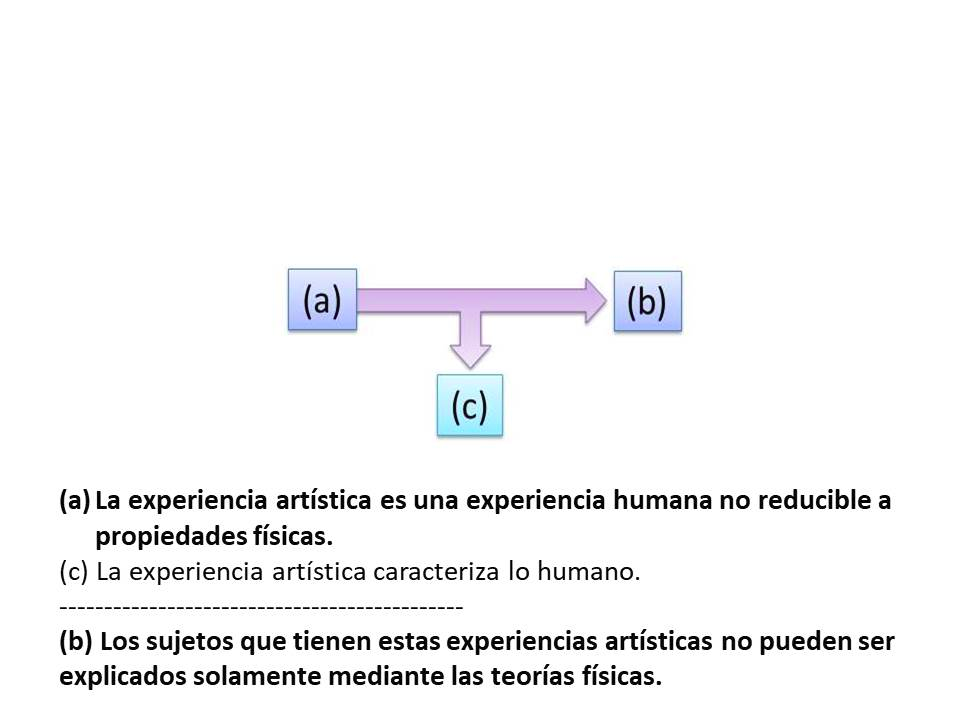
\includegraphics[width=5.76744in,height=2.86101in]{media/image2.png}

\end{center}

Si logramos aceptar (a) y (c) no tendremos razones para dudar de (b).
Así las cosas, en primer lugar, se explicará cómo la experiencia
artística caracteriza lo humano. En segundo lugar, se mostrará como la
explicación física no logra abarcar la riqueza de la experiencia
artística eliminando del Argumento de Conocimiento de Frank Jackson la
postulación de los \emph{qualia} (propiedades subjetivas de la
experiencia) y proponiendo en su lugar el punto de vista subjetivo del
que habla Thomas Nagel. Y, en tercer y último lugar, se verá como la
aceptación de estas premisas trae problemas al proyecto fisicalista en
la medida en que este niega que los sujetos que tienen estas
experiencias artísticas no puedan ser explicados solamente mediante las
teorías físicas.

\section*{I. La experiencia artística caracteriza lo humano.}

Un ser humano es un ser de experiencias y eso define su identidad, su
carácter racional, pues es difícil concebir un ser humano racional y sin
experiencias. Parece que la experiencia artística hace parte de las
experiencias que definen lo humano. Uno quizá puede decir que la
experiencia artística es la manera correcta de presenta/especificar la
experiencia humana (experiencia con objetos/personas/sí mismo) pues
aunque no todos estén llamados a ser artistas en el sentido específico
de la palabra, cada hombre en la medida en que es artífice de la propia
vida puede hacer de ella una obra de arte, una obra maestra (\cite{Juan1999}).

La experiencia artística es, entonces, la interpretación que hace el ser
humano de un conjunto de palabras escritas y orales, de manifestaciones
teatrales y musicales, de expresiones de las artes plásticas y de las
más modernas tecnologías de la comunicación. La experiencia artística,
aunque puede necesitar del objeto físico no se agota en este; una
escultura a pesar de ser una manifestación del arte plástico no es
suficiente para que se hable de experiencia artística pues aún no se
encuentra en relación con alguien. La experiencia artística caracteriza
lo humano en la medida en que permite que el hombre se apropie de lo que
lo rodea, lo interprete. La experiencia perceptual es el soporte de la
relación que tiene el hombre con lo que lo rodea, pero es insuficiente
para dar cuenta de la experiencia humana si se le desvincula de la
experiencia artística como esa capacidad de interpretar lo que está
alrededor. Al ser humano que contempla no le basta percibir, sino que
irremediablemente interpreta, la experiencia artística permite al hombre
ir más allá de colores, formas o sonidos de quien contempla o escucha.
Resulta complicado imaginarse un caso de una persona que carezca de
experiencias artísticas precisamente porque estas son un rasgo propio
del hombre para relacionarse consigo mismo, con el mundo y con los
demás. Basta con un sentido para que el hombre pueda tener una
experiencia artística de alguna clase. El ser humano parece ser una
subjetividad dotada de un mundo interior, que tiene sus pensamientos y
elecciones, sus afectos y relaciones, sus proyectos e ideales. El ser
humano es tan complejo que parece que no es posible caracterizar su
subjetividad mediante propiedades físicas, cosa que sí logra hacer la
experiencia artística como veremos a continuación.

\section*{II. La explicación física no logra abarcar la riqueza de la
  experiencia artística}


Cada organismo tiene una forma propia de tener experiencias conscientes
y es por ello que muchas experiencias están directamente relacionadas
con un solo punto de vista: el del organismo que tiene la experiencia.
Esto ocurre en la medida en que hay algo que es ser un murciélago, un
hombre, un marciano--o lo que se quiera. Ese modo de ser, para el
organismo que elijamos, está ligado a un punto de vista particular. Así,
este punto de vista particular no se puede transferir a otro, es una
suerte de perspectiva en primera persona que no se puede compartir así
el otro haya experimentado lo mismo. Thomas Nagel, en su artículo
\emph{¿Cómo es ser un murciélago?,} lo ejemplifica maravillosamente
diciendo que un murciélago tiene experiencias conscientes en el sentido
de que hay algo que es cómo se siente tal experiencia para el
murciélago, es decir, que hay algo que es cómo es ser un murciélago para
el murciélago. Para Nagel, lo que constituye la manera de ser de un
organismo son las experiencias que éste tiene, las cuales están
determinadas (al menos en parte) por los aparatos perceptuales de ese
organismo. Ahora bien, nuestras capacidades imaginativas están
restringidas por nuestras experiencias y recursos mentales, y es por
ello que la imaginación, por mucho que se esfuerce, es demasiado
limitada a la hora de saber lo que es ser como un murciélago pues no
tenemos ningún sentido que se parezca a la ecolocación de un murciélago.

Una persona sólo puede saber o decir cuál es la cualidad de la
experiencia de otra en la medida en que ese alguien ``sea lo
suficientemente similar al objeto de la atribución como para poder
adoptar su punto de vista'' (\cite{Nagel2003}), pero nunca podrá dar cuenta de ella
totalmente porque la experiencia no es del todo objetiva. Es por esta
razón que, aunque pueda imaginarme que tengo los rasgos de un murciélago
(que tengo alas, que vuelo al atardecer, que como fruta, que tengo muy
mala visión), esto no sería imaginar cómo es ser un murciélago para un
murciélago, sino cómo sería, para mí ser un murciélago. Si los hechos de
la experiencia son sólo accesibles desde un punto de vista, entonces
resulta un misterio cómo una explicación física objetiva o independiente
de ese punto de vista puede dar cuenta de las experiencias. Así, ninguna
cantidad de información física puede decirnos cómo es ser murciélago
debido a que el cómo es ser algo sólo se puede entender desde el punto
de vista del murciélago, y a eso no podemos acceder desde nuestro punto
de vista.

En el caso de la experiencia artística el punto de Nagel se aplica a la
perfección. Es muy cierto que hay una parte de este tipo de experiencias
que podemos entender en términos objetivos: los sonidos, los ritmos, las
palabras, los colores se pueden medir y captar hasta cierto punto
mediante procedimientos científicos, hay teorías que buscan explicar
este tipo de experiencias a partir de propiedades físicas. No obstante,
como bien muestra Nagel, entender la experiencia desde sólo ese aspecto
no logra capturarla en su totalidad. La parte subjetiva de la
experiencia artística ``brota de lo más íntimo del alma humana, allí
donde la aspiración a dar sentido a la propia vida se ve acompañada por
la percepción fugaz de la belleza y de la unidad misteriosa de las
cosas'' (\cite{Juan1999}). Cada experiencia artística tiene una manera de ser y sentirse
propia que no puede atraparse en lo físico, ya que los términos físicos
deben ser comprendidos por igual desde muchos puntos de vista, lo cual
perdería validez cuando se acepta la existencia de un punto de vista
particular. Es posible caracterizar la experiencia artística en general,
incluso explicar qué sentimientos puede generar la obra \emph{La
resurrección} de Gustav Mahler o el \emph{David} de Miguel Ángel, sin
embargo, no resulta fácil explicar cómo se siente para alguien esta
experiencia artística.

El argumento de Nagel, empero, tiene una falencia: que la subjetividad
de la experiencia puede entenderse totalmente en términos de un
saber-cómo (\emph{know-how}), de un tipo de saber particular. Sobre este
punto habla David Lewis\footnote{En su artículo \emph{Lo que enseña la
  experiencia}} afirmando que lo que se adquiere cuando se experimenta
por primera vez una sensación no es conocimiento proposicional sino una
capacidad recognoscitiva. El cómo se siente está relacionado más a la
adquisición de unas nuevas habilidades que a la experiencia en sí, al
conocimiento de hechos. De acuerdo con la hipótesis de la habilidad de
Lewis, el carácter subjetivo se reduce a habilidades de imaginar,
reconocer y recordar (\cite{Lewis2003}). A pesar de que Lewis comienza teniendo un muy buen
punto, parece que una persona necesita de la experiencia para poder
reconocer, imaginar y recordar, no parte nunca de cero. Aunque nos es
posible imaginarnos, reconocer o recordar una experiencia, esto sólo se
convierte en posibilidad si ya hemos experimentado en primera persona
ese cómo se siente. En el caso de que sea una experiencia ajena, sólo
podremos acercarnos un poco a ese cómo se siente si somos
suficientemente similares al objeto de la atribución como para poder
adoptar su punto de vista.

Una manera fuerte de mostrar como la hipótesis de la habilidad de Lewis
no es suficiente para explicar la parte subjetiva de la experiencia (ese
saber cómo se siente tener una experiencia) es el Argumento de
Conocimiento de Frank Jackson\footnote{En su artículo \emph{What Mary
  did not know.}}. Éste describe a una brillante científica llamada
Mary, quien tiene conocimientos científicos completos, es decir, sabe
todo lo que hay que saber en términos físicos (incluyendo todo lo que
hay que saber acerca del color). Ella, sin embargo, se ve obligada a
investigar el mundo desde una habitación en dónde todo se ve a blanco y
negro, su cuerpo, los libros y la televisión. En un determinado momento,
Mary sale de la habitación y ve por primera vez un tomate, al hacerlo,
se da cuenta que había algo que no sabía: el cómo se siente ver algo
rojo pues nunca había experimentado la sensación de color. La falta de
conocimiento de Mary no se resolvió imaginándose qué serían los colores,
tampoco se suplió con inferencias lógicas, ``lo que directamente viene
al caso no es la clase ni la manera ni el tipo de conocimiento que tiene
Mary, sino lo que sabe'' (\cite{Jackson2003}), Mary, aunque sabía todo lo físico e incluso,
de acuerdo con Lewis, tenía la habilidad de imaginar todo lo que existe,
al salir al mundo exterior y tener por primera vez una experiencia
particular, sabe algo nuevo acerca del mundo, conoce el color, y se da
cuenta de que la concepción que tenía de la vida mental de los otros (y
de ella) estaba muy empobrecida. Mary sabía acerca de los \emph{qualia}
de negro (o de ciertos tonos de gris), empero, no sabía nada acerca del
\emph{qualia} de rojo. Mary tenía todo el conocimiento sobre el color
rojo, pero carecía de esa característica subjetiva de la experiencia de
rojo.

Ahora bien, el Argumento de conocimiento funciona muy bien, pero, al
igual que el de Nagel presenta un problema, a saber, la postulación de
los \emph{qualia.} Los \emph{qualia} presentan diversos problemas debido
a que no son sólo vagos o equívocos, sino que son profundamente
confusos. La indefinición de los \emph{qualia} se da en la medida en que
al final es la opinión del sujeto el criterio último para decidir
respecto a los qualia de sus experiencias (a pesar de que la pretensión
original cuando se esbozan los qualia es la de englobar lo que tiene de
subjetiva la experiencia). Los defensores de los \emph{qualia} los
definen como unas características intrínsecas ya que no cambian
dependiendo de la relación de la experiencia con otras cosas, sin
embargo, lo que tratan de mostrar filósofos como Daniel Dennett es que
estos si varían con la repetición de una misma experiencia u otras
diferentes. Así se explica el desarrollo de un gusto por ciertas bebidas
con la ingestión repetitiva de la bebida en cuestión, o como la
fenoltiourera (un tipo de sustancia) tiene un sabor muy amargo para tres
cuartas partes de la humanidad mientras que para el resto es sinsabor
(Dennett, 2003). El amargo o el gusto o disgusto que producen ciertos
alimentos no constituyen una propiedad intrínseca de las cosas sino una
propiedad relacional.

Parece que los \emph{qualia} surgen porque se busca dar cuenta de la
manera en la que se siente algo. También parece que esos qualia son
inefables, intrínsecos, privados y directamente aprehensibles en la
conciencia, y es por ello que si yo quisiese explicar a alguien lo que
se siente comer la arepa que hace mi abuela no sólo es que sea difícil
que la otra persona me entienda, sino que incluso ni yo misma sé por
dónde comenzar a explicarla. Los \emph{qualia}, esas cualidades
subjetivas que se postulan tratando de explicar esa naturaleza subjetiva
de la experiencia, no resultan exitosos, esas ``propiedades inefables,
intrínsecas, privadas y directamente aprehensibles de la experiencia
(\ldots{}) En su lugar {[}solamente{]} encontramos propiedades públicas
relativas o prácticamente inefables a las que podemos referirnos de
manera indirecta por referencia a nuestros detectores de propiedades
privadas'' (Dennett, 2003, p. 258). No obstante, este logro de Dennett
al mostrar la dificultad que existe en nombrar lo subjetivo de la
experiencia bajo la postulación de los \emph{qualia} no logra anular la
posibilidad que haya algo subjetivo en la experiencia.

De este modo, buscando eliminar los defectos y potenciar las bondades de
tanto el argumento de Nagel como el de Jackson, se plantea eliminar del
Argumento de Conocimiento la postulación de los \emph{qualia}
proponiendo en lugar de estos el punto de vista subjetivo del que habla
Nagel. Así, imaginemos entonces que le mostramos una partitura a Mary
(que es ahora directora de orquesta) y esta puede imaginarse como
sonaría la pieza. Una partitura es la expresión escrita de cómo debe
sonar una pieza. En la partitura encontramos una clave, que nos dice en
qué alturas están las notas, unas figuras, que nos dicen que ritmo debe
tener cierta melodía y, además, nos dicen con exactitud qué notas deben
tocarse en cierta parte determinada. También encontramos unas dinámicas
que nos dicen qué tanto volumen debe tener esa parte de la obra, hay una
métrica que establece el compás de la obra, también la partitura nos
dice cuántas negras debe haber por minuto, hay también unas intenciones,
que nos dicen cómo, por ejemplo, debe tocarse el arco para obtener
cierto sonido y, además, encontramos una tonalidad. Así, antes de
ensayar con una orquesta, podemos decir que Mary ya sabe cómo debería
sonar la obra. Sin embargo, a este formato, aunque logre abarcar el cómo
suena la pieza, no logra contener la totalidad de la experiencia
artística porque no deja lugar a la interpretación. Al igual que en el
Argumento de Conocimiento, cuando Mary escucha la obra en un concierto
se da cuenta que su conocimiento físico no logra abarcar la experiencia
artística en su totalidad, hay algo que se escapa a la descripción
física que va más allá del ritmo y la tonalidad, que está en el sujeto
que escucha, que toca.

¿Qué es lo que no conoce? Efectivamente, como dicen Jackson y Nagel, es
la parte subjetiva de la experiencia, pero esta parte subjetiva no se
entiende a partir de los \emph{qualia} que postula Jackson, sino a
partir del punto de vista particular que defiende Nagel. Mary al oír el
concierto y tener por primera vez esta experiencia enriquece lo que sus
sentidos conocen, y, en la medida en que las experiencias están
determinadas (al menos en parte) por los aparatos perceptuales de un
organismo, entonces Mary está en posición de entender mejor su vida
mental. A Mary no le bastó su conocimiento de términos físicos para
saber cosas acerca del mundo, necesitó enfrentarse con la experiencia
personalmente, es por ello que muchas veces ``los artistas tienen en
común la experiencia de la distancia insondable que existe entre la obra
de sus manos, por lograda que sea, y la perfección fulgurante de la
belleza percibida en el fervor del momento creativo'' (\cite{Juan1999}).

\section*{III. El fin del proyecto
  fisicalista: El ser humano no puede ser explicado solamente mediante
  las teorías físicas.}


Ya que se ha logrado mostrar que si (a) la experiencia artística es una
experiencia humana no reducible a propiedades físicas \emph{entonces},
no hay ningún reparo en afirmar que (b) los sujetos que tienen estas
experiencias artísticas no pueden ser explicados solamente mediante las
teorías físicas. La comprobación de esta hipótesis choca de lleno con el
proyecto fisicalista, pues este sostiene la tesis de que la persona no
es nada más que su cuerpo y todas sus propiedades físicas. Los
promotores de este proyecto son quienes dudan respecto al carácter
subjetivo de la experiencia porque piensan que todo puede ser descrito
en términos objetivos, ya que todo lo que existe es físico. El
fisicalismo explica muchas cosas y por ello no se busca negar, bajo
ningún pretexto, la parte objetiva de la experiencia; la ciencia
funciona, y puede, o podrá en algún momento dar cuenta de todas las
cosas físicas que existen. Pero, la experiencia artística va mucho más
allá de la percepción, a partir de una serie de manifestaciones
artísticas como la música, la pintura y la poesía se logre atrapar mucho
más que lo físico en los paisajes y sonidos.

El problema del proyecto fisicalista es que su pretensión es
totalitaria, porque cree que todo se puede explicar mediante propiedades
físicas, y la ventaja de rechazarlo, es que se abre la puerta a
explicaciones del mundo de carácter no-físico. El rechazo del
fisicalismo no lleva a afirmar la creencia en cosas o seres
inmateriales, tampoco hace que sea válido o razonable hablar de temas
como Dios y el alma en el sentido cristiano de la palabra; solamente
deja abierta la posibilidad de existencia de estos elementos en tanto
que, si no bastan las propiedades materiales para explicar al hombre,
puede que haya otro tipo de cosas que tampoco se puedan explicar
mediante estas propiedades. Así, la belleza puede verse como la clave
del misterio y la llamada a lo que va más allá de las cosas tangibles y
que caben en la lógica fría y discursiva.


\nocite{BarriosRuiz2014}
\nocite{Dennett2003}
\nocite{Murray1979}
\nocite{Nagel1965}
\nocite{RomeraSF}

\printbibliography[heading=subbibliography,title={Referencias}]

\end{refsection}




\begin{refsection}
\chapter{\texorpdfstring{\textbf{Objetos intensionales como criterios de
identidad de las
experiencias.}}{Objetos intensionales como criterios de identidad de las experiencias.}}\label{objetos-intensionales-como-criterios-de-identidad-de-las-experiencias.}

\autor{Juan Manuel Gaitán\footnote{Estudiante de sexto semestre de
  Filosofía de la Universidad de La Sabana. Correo:
  \href{mailto:juanga@unisabana.edu.co}{\nolinkurl{juanga@unisabana.edu.co}}}}

A medida que han ido surgiendo teorías que intentan explicar las
experiencias como hechos importantes en la comprensión de la mente o el
cerebro, ha surgido también la preocupación por determinar o reconocer
cuándo podemos decir que las experiencias son iguales o son las mismas.
Aquello que nos permita determinar cuándo las experiencias son iguales o
las mismas, lo llamaremos criterios de identidad de las experiencias; La
identidad sobre la que hablamos es de tipo (\emph{type}) y no de caso
(\emph{Token}). Es así como siempre que hable de identidad y criterios
de identidad a lo largo de este escrito, me referiré a identidad-tipo de
las experiencias. Cabe resaltar que decimos que una experiencia es igual
a otra o la misma cuando pertenecen a la misma clase de experiencia;
esto es, dos experiencias de comer piña serán iguales en la medida en
que pertenezcan a la misma clase de experiencia, a saber, comer piña.
Pienso que es importante exigir a las teorías que intentan explicar la
percepción que tengan criterios claros para la identidad de las
experiencias. Parece que, si bien podemos deducir las respuestas del
fisicalismo y el funcionalismo, los qualia sin embargo son un poco
oscuros al respecto. Podría argumentarse que un estado de dolor es el
mismo cuando sus qualia respectivos, o el ``cómo se sienten'', son
iguales. Sin embargo, esto no es del todo claro.

Dennett nos pone un ejemplo bastante ilustrativo. Yo detesto la
coliflor, sin embargo, he comprado una pequeña pastilla que al tomarla
hará que me guste la coliflor. Al tomar la pastilla surte efecto, la
siguiente vez que comí coliflor me sabía exquisito. Tenemos un problema.
Tengo varias opciones para explicar el fenómeno. Podría decir que la
pastilla no ha cambiado el sabor de la coliflor, pues no ha hecho que
sepa a chocolate, el cambio ha sido en mí. Tengo aún varias opciones.
1). Podría ser que el quale no cambió y de hecho el sabor de la coliflor
es igual, fueron mis gustos los que cambiaron. 2). En realidad el quale
de la coliflor cambio por lo cual mis gustos también lo hicieron. 3). Ni
el quale ni mis gustos cambiaron, sólo mi acceso a las memorias del
sabor de la coliflor se vio afectado y recuerdo el sabor de manera
diferente, aunque de hecho es el mismo. La pregunta que surge es obvia
¿el sabor de la coliflor es el mismo quale de antes de que me tomara la
pastilla? ¿Bajo qué criterio puedo definirlo? (Dennett, 2003, p. 217).

Pongamos otro ejemplo expuesto por Dennett. Más que un ejemplo es un
aspecto interesante sobre uno de los problemas expuestos en ``Quining
qualia'' de D. Dennett. Dennett (2003) nos dice que el primer sorbo de
jugo de naranja del desayuno puede saber diferente del segundo si los
intercalo con un bocado de panqueques con miel. Seguramente todos hemos
notado que el sabor del jugo cambia al haber comido algo más dulce breve
tiempo antes. Podríamos preguntarnos ¿es el mismo quale en el primer y
segundo sorbo? Quizá no sea un gran problema la pregunta, fácilmente se
podría responder que, al añadirle el elemento extra de la miel y el
panqueque, por supuesto que es un quale diferente. Pero esto es un
problema ¿Qué elementos deben tomarse en cuenta y cuales no al momento
de la percepción y de definir cuál es el quale de dicha percepción?
Pongamos un ejemplo que ilustre nuestro punto: Supongamos que cada día
todos los días me tomo una deliciosa taza de chocolate caliente. Llevo
haciéndolo ya durante varios años, evidentemente me encanta el chocolate
caliente. Sin embargo, un día ya no quiero mi taza diaria de chocolate,
estoy hastiado de tanto chocolate durante tanto tiempo, ya no me agrada,
no en la forma que lo hacía antes. Hagamos la misma pregunta ¿Sigue
teniendo el mismo quale, la misma experiencia que cualquier otro día que
tomé la taza de chocolate caliente? Supongamos que sí. Por la forma en
la que hablé podemos decir que si, quizá sí sigue siendo el mismo quale.
Lo único que cambió fueron mis gustos o la forma en la que reacciono
frente a ese quale específico. Sin embargo, al contarle a mi novia, ella
me revela una posibilidad que no había pensado, a saber, que
evidentemente el chocolate no sabe igual, de la misma manera que
siempre, pues en el momento en que he ingresado un nuevo elemento a la
percepción, a saber, el desagrado, ya no era la misma experiencia de
siempre, había un elemento extra.

Si estamos dispuestos a aceptar el caso del jugo de naranja y el
panqueque ¿por qué este caso sería diferente? ¿Cuál es el criterio para
discriminar elementos que convergen en la percepción que en ocasiones
consideramos como cambiantes de la percepción misma y en otras ocasiones
eliminamos elementos y no los consideramos como elementos esenciales de
la percepción?

Es evidente que existe un problema en la teoría de los qualia. Este será
el problema que intentaremos resolver: Los criterios de identidad bajo
los cuales podemos determinar que una experiencia es igual a otra.
Cuando el sabor del chocolate es el mismo en diferentes momentos de
tiempo bajo diferentes circunstancias. Evidentemente esta tarea no será
sencilla. Por esto me apoyaré en ``La cualidad intrínseca de la
experiencia'' por Gilbert Harman. A partir de Harman (2003), intentaré
dar una posible solución a los problemas planteados por Dennett y
mencionados anteriormente respecto de los qualia.

Debemos en primer lugar justificar en qué medida podemos identificar las
propiedades intrínsecas de Harman con los qualia. Para esto usaré la
caracterización que hace Dennett de estos y a partir de ahí justificar
por qué las identifico.

Para Harman, las propiedades intrínsecas de la experiencia son
simplemente el ``cómo es'' tener una experiencia (esto, por supuesto, en
las palabras de Nagel, 2003, p. 46). Sin embargo, Harman no ofrece una
concepción más detallada de lo que esto significa, pues su punto no es
refinar la idea de propiedades intrínsecas de la experiencia. Su
objetivo es mostrar que esto no es un problema para una teoría que da
cuenta de las experiencias. Sin embargo, creo que esta caracterización
de dichas propiedades es suficiente para identificarlos con los qualia
entendidos de una forma muy elemental. Dennett (2003, p. 213), en
``Quinear los qualia'', nos dice que según la jerga filosófica
tradicional los qualia son caracterizados como \emph{la manera en que
nos parecen las cosas}. Los qualia son propiedades subjetivas
intrínsecas de la experiencia, es el \emph{cómo a ti te parece}. Imagina
que un día caluroso decides comer trozos de una jugosa piña. El sabor
particular de la piña es un quale gustativo. El color particular de la
piña es un quale visual de la piña.

Es esto por lo que considero que se puede identificar las propiedades
intrínsecas de las que habla Harman con los qualia en la manera
caracterizada por Dennett. Es por esto que a lo largo de este texto
hablaré de qualia y propiedades intrínsecas tratándose de la misma cosa.

Para resolver este problema es necesario introducir el concepto de
\emph{intencionalidad} pues este nos permitirá zanjar el problema o al
menos dar una posible solución. Harman nos da dos argumentos para
entender la intencionalidad.

\begin{enumerate}
\def\labelenumi{\arabic{enumi}.}
\item
  Ponce de León está buscando la fuente de la juventud.

  No existe algo como la fuente la juventud.

  Pero no se sigue que Ponce de León no buscase nada.
\end{enumerate}

Podemos decir que La búsqueda de Ponce de León tiene un objeto
intensional que, aunque de hecho no exista no implica que Ponce de León
no buscase nada.

\begin{enumerate}
\def\labelenumi{\arabic{enumi}.}
\item
  ``Es importante distinguir entre las propiedades de un objeto
  representado y las propiedades de una representación de dicho objeto''
  (Harman, 2003, p. 273). Imagine que usted está viendo la pintura de un
  unicornio. Puede ver la pintura sobre el óleo, los diferentes colores
  de las pinturas usadas, etc. Compare la pintura del unicornio con la
  representación o la imagen que tiene usted de un unicornio en su
  imaginación. Es claro que en ambos casos el objeto es el mismo y que
  además este no existe. Es importante que distinga, sin embargo, entre
  las cualidades del objeto de su representación (la imagen que tiene
  del unicornio en su ``mente'') y la representación del objeto (la
  pintura del unicornio). La representación que usted tiene de seguro no
  comparte las mismas propiedades que la pintura, aunque ambas sean del
  mismo objeto. La pintura se presenta como plana y cubierta de pintura.
  Su representación del unicornio no es ni plana ni está cubierta de
  pintura, etc.
\end{enumerate}

Este argumento señala dos cosas importantes: 1). Es importante la
distinción entre las propiedades de un objeto representado y las
propiedades de la representación misma. 2). El objeto de representación
no necesariamente debe existir para ser objeto de representación. Esto
lo llamaremos objeto intensional.

¿Cómo enfrentamos los problemas de Dennett sobre los qualia desde
Harman?

Lo primero que debemos decir frente a los qualia es que hay un error de
distinción. La concepción de los qualia surge a partir de la distinción
que se hace entre la experiencia y el objeto de la experiencia. Pienso
que no somos capaces de abordar la experiencia misma independiente de su
objeto para hablar de sus propiedades intrínsecas. Es decir, no se puede
separar el objeto intensional de la experiencia de la experiencia misma.
Así, cuando hablamos de propiedades intrínsecas de la experiencia en
realidad hablamos de propiedades del objeto intensional. Esto ya no
resulta un problema, al menos para los criterios de identidad de las
experiencias, porque podremos dar cuenta de las experiencias
funcionalmente teniendo en cuenta las relaciones entre las entradas (los
órganos por los que percibimos), las salidas (las conductas que se
generan como reacciones) y los objetos intensionales de la experiencia.
Si se desea saber cuáles las propiedades intrínsecas del objeto
intensional o el quale de cada objeto, deberá buscar en otra teoría que
se encargue acerca de las propiedades de los objetos. No es un problema
para nosotros en la medida en que solo debemos dar cuenta de las
relaciones funcionales de las experiencias.

Ahora sí debemos dar una respuesta a los criterios de identidad de las
experiencias. Ya hemos mostrado que los qualia no son propiedades
pertinentes de las cuales una teoría de la experiencia deba dar cuenta,
pues los qualia son, al menos, propiedades intrínsecas del objeto
intensional y no de la experiencia misma. Por esto los qualia no pueden
ser el criterio bajo el cual una experiencia es igual a otra.
Expliquemos esto.

Según algunas teorías de los qualia estos son criterios de identidad de
las experiencias, es decir que el qualia es el que determina la
experiencia que tengo. Por ejemplo, yo me encuentro en un estado de
dolor cuando tengo el mismo carácter cualitativo o qualia de dolor,
podemos llamarlo quizá lo doloroso del dolor. Retomando el ejemplo de la
piña podríamos decir que tengo la misma experiencia de comer piña cuando
el qualia es el mismo, a saber, el \emph{cómo sabe para mí} de la piña
es igual (Shoemaker, 2003, p. 184).

Los qualia no pueden sernos útiles para identificar experiencias, pues
son propiedades del objeto. Pero sólo son unas de varias propiedades del
objeto y no es muy claro porque razón elegiríamos esas propiedades y no
otras del objeto para identificar las experiencias. Por esto creo que lo
más adecuado es tomar todo el objeto intensional como criterio de
identidad de las experiencias. Es decir, tendré una experiencia de piña
siempre y cuando el objeto intensional de mi percepción sea una piña.
Creo que el objeto intensional es un buen criterio en la medida en que
puedo \protect\hypertarget{_Hlk508645306}{}{}identificar las diferentes
experiencias funcionalmente teniendo en cuenta las entradas, ya sean
terminaciones nerviosas (dependiendo de lo refinadas que se quieran las
entradas) o el objeto externo, las salidas o conductas que pueden
generar las experiencias y su relación con los objetos intensionales de
las experiencias.

Referencias

Dennett, D. (2003). Quinear los qualia En M. Ezcurdia y O. Hansberg
(Comps.), \emph{La naturaleza de la experiencia} (Vol. 1: Sensaciones)
(213-262).

Harman, G. (2003). La cualidad intrínseca de la experiencia. En M.
Ezcurdia y O. Hansberg (Comps.), \emph{La naturaleza de la experiencia}
(Vol. 1: Sensaciones) (263-288).

Nagel, T. (2003). ¿Cómo es ser un murciélago?. En M. Ezcurdia y O.
Hansberg (Comps.), \emph{La naturaleza de la experiencia} (Vol. 1:
Sensaciones) (45-64).

Shoemaker, S. (2003). Funcionalismo y qualia. En M. Ezcurdia y O.
Hansberg (Comps.), \emph{La naturaleza de la experiencia} (Vol. 1:
Sensaciones) (183-212).

\nocite{Dennett2003}
\nocite{Harman2003}
\nocite{Nagel2003}
\nocite{Shoemaker2003}


\printbibliography[heading=subbibliography,title={Referencias}]

\end{refsection}



\chapter{\texorpdfstring{\textbf{Sobre el estatus ontológico de la improvisación musical}}{Sobre el estatus ontológico de la improvisación musical}}\label{sobre-el-estatus-ontológico-de-la-improvisación-musical}

\autor{Tatiana Gómez Sánchez\footnote{Estudiante de séptimo semestre de
		Filosofía de la Universidad de La Sabana. Correo:
		\href{mailto:tatianagosa@unisabana.edu.co}{\nolinkurl{tatianagosa@unisabana.edu.co}}} \footnote{Agradezco a Dios.\\
		Este trabajo, fruto del estudio en \textit{Metodología de la Investigación}, fue presentado en el \textit{I Foro interno del semillero de investigación en Ciencia, Lógica y Metafísica} de la Universidad de La Sabana y en el \textit{II Congreso de Lógica y Epistemología Contemporánea} en la Universidad Nacional de Colombia. Agradezco los comentarios que recibí, especialmente al doctor Axel Barceló, y los aportes de mis profesores y maestros. Agradezco a mis compañeros de Metodología, en especial a Paula Sierra, Juan Manuel Gaitán, Cristian González y Miguel Prieto. Así como también a Pablo Rivas, Camila Sarmiento, Daniela Henao y a mi familia.\\
		Agradezco al profesor Juan Camilo Espejo-Serna por su asesoría y apoyo.}}

\section*{Introducción}

Una parte del debate contemporáneo sobre la filosofía de la música gira
en torno a la ontología musical, que principalmente estudia el estatus
ontológico de una obra musical, es decir, qué es una obra musical, y la
relación que esta mantiene con sus performances\footnote{Performance lo
  voy a entender como la actividad ejecutoria de una pieza musical, por
  medio de una secuencia de sonidos.}. Hay una noción que permite y se
ha usado para explicar estas dos cuestiones, y es la distinción
tipo/caso, según la cual la obra es un tipo que se instancia o se repite
en performances (casos).

La improvisación musical, caracterizada por ser una actividad
espontánea, efímera, irrepetible, incorregible y libre, de hacer música;
es una cuestión que presenta varios desafíos para la ontología musical,
pues, teniendo en cuenta las características de la improvisación resulta
difícil concebirla como una obra musical. Y en especial resulta difícil
concebirla como una obra bajo la distinción tipo/caso, como más adelante
explicaré. Teniendo en cuenta esto, en esta ponencia no solo buscaré dar
respuesta a la siguiente pregunta: ¿es posible escuchar de nuevo y en
vivo una misma improvisación musical?, al decir que sí es posible en un
sentido, sino que también, a partir de la respuesta que daré, presentaré
una forma de abarcar un problema relevante en el debate actual de la
ontología musical, a saber, concebir la improvisación musical como una
obra.

La cuestión que aquí trabajo es de tipo interdisciplinar, porque, por un
lado, tiene un carácter filosófico, y, por otro lado, porque resulta
pertinente para el estudio de la música, y del arte mismo. Dado que el
tema de la ponencia es el estatus ontológico de la improvisación
musical, me limitaré a hablar acerca de lo que \emph{es} una
improvisación musical y por tanto no voy a responder preguntas sobre
cómo podría llegar a ser posible producir una misma improvisación
musical, ni cómo es posible para un oyente \emph{reconocer} una
improvisación musical como la misma. Quiero ofrecer una base ontológica
sobre la cual, quizá, luego responder ese tipo de preguntas.

Así, el orden que seguiré en esta ponencia será el siguiente: (I)
caracterización de la improvisación musical, (II) la distinción tipo/caso
como herramienta de la ontología musical para caracterizar una obra y su
relación con el performance, (III) dos sentidos en los que se puede
entender que una pieza musical sea la \emph{misma}, (IV) concebir la
improvisación como una obra musical a partir de la distinción tipo/caso,
y (V) respuesta a la pregunta y la pertinencia del tema en el debate de
la ontología musical.

\section*{I. Improvisación musical}


La improvisación musical ha sido caracterizada como una actividad
espontánea, efímera, irrepetible, singular, incorregible y libre, de
hacer música (Alperson 1984-2010, Bertinetto 2012, Brown 1996, Davies
2001-2011), en la que las decisiones de los músicos tienen ciertas
características. El improvisador se encuentra en una \textbf{situación}
que se caracteriza por construir sobre los pasos que acaba de tomar, a
diferencia del compositor ordinario que puede borrar movimientos y
volver a escribirlos; tiene que tomar \textbf{decisiones forzadas} en la
que no puede tomar tiempo para pensar y corregir, sino que debe hacer
algo en el momento, de inmediato (Brown, 2000). Y las decisiones acerca
de cómo y de qué tocar no dependen de instrucciones previas, el
improvisador no tiene un \textbf{guion}, una guía o direcciones
especificas acerca de cómo hacer el performance. (Brown 2000; Bertinetto
2012). No obstante, esto no quiere decir que las decisiones y elementos
de una improvisación sean creadas \emph{ex nihilo}, pues los músicos
improvisan sobre fórmulas, patrones y estilos artísticos (Alperson 1984,
Bertinetto 2012, Brown 1996, Young and Matheson 2000, Davies 2001, Kania
2011).

\section*{II. Distinción tipo/caso y el estatus ontológico de una obra
  musical}


La distinción entre un tipo y sus casos es una distinción ontológica
entre un tipo general de cosas y sus instancias particulares y
concretas, por ponerlo en una forma preliminar e intuitiva (Wetzel,
2014). En estética usualmente es preciso distinguir entre las obras de
arte (tipos) de sus ``productos'' concretos o encarnaciones físicas
(casos) (Wollheim 1968; Wolterstorff 1980; Davies 2001). Puede haber más
de un solo caso de una escultura hecha de un molde, más de una copia de
una película, y más de un performance de una obra musical.

Propiamente en la música, la distinción tipo/caso se usa para determinar
lo que es una obra musical, y para dar cuenta de la relación entre la
obra (tipos) y sus performances (casos). En otras palabras, esta
distinción es una de las herramientas básicas para entender el carácter
ontológico de la obra musical y para dar cuenta de la relación entre la
obra (tipos) y sus performances (caso). Según esto una pieza musical es
considerada una obra musical en virtud de su carácter repetible, es
decir, en virtud de que se repita o se instancie en casos particulares.

Una de las mayores problemáticas que aquí se presenta consiste en
introducir la noción de improvisación musical, en tratar de concebirla
como una obra musical a partir de esta distinción, porque la
improvisación se caracteriza por ser, efímera, irrepetible, incorregible
y espontánea; aspectos que parecen ir en contra del carácter repetible
que presenta la distinción tipo/caso. Entonces, o bien decimos que la
improvisación musical no es una obra musical o bien ofrecemos una
caracterización de la improvisación que sí sea compatible con la
distinción tipo/caso. En lo que sigue ofreceré una posible salida.

\section*{III. Distinción \emph{mismo\textsubscript{1}} y
  \emph{mismo\textsubscript{2}}}


Puesto que la pregunta es acerca de si es posible o no escuchar de nuevo
y en vivo una misma improvisación musical, a continuación, presento dos
formas en las que hasta ahora encuentro que se puede hablar de una
\emph{misma} pieza musical. Un primer sentido, llamémoslo
\emph{mismo\textsubscript{1}}, consta de las condiciones
espacio-temporales de una pieza musical. Un segundo sentido,
\emph{mismo\textsubscript{2}}, se refiere a la estructura sonora de la
obra, a cuestiones como la melodía, armonía, adornos, estructura
musical, tempo y ritmo, etc.

En el siguiente ejemplo busco explicar la distinción tipo/caso bajo la
cual se explica lo que es una obra y su relación con sus performances y
la distinción de \emph{mismo} que hasta ahora he expuesto.

Ejemplo: la \emph{Quinta Sinfonía} de Beethoven.

Esta pieza musical se concibe como una \emph{obra}, compuesta entre 1804
y 1808, y estrenada en ese último año. No obstante, la \emph{Quinta
Sinfonía} no solo se interpretó una vez sino que, de hecho, se han hecho
distintos performances de ella hasta llegar a nuestros días. Así, es una
obra que se ha repetido con el paso del tiempo en distintos
performances, por poner un ejemplo, en un teatro de nuestra ciudad la
semana pasada. Sin embargo, hay un sentido en el que estos performances
interpretan la \emph{misma\textsubscript{2}} obra musical, y otro
sentido (\emph{mismo\textsubscript{1}}) en el que no lo hacen. Por un
lado, sí interpretan la \emph{misma\textsubscript{2}} obra en cuanto a
que tocan la composición de Beethoven, siguen sus instrucciones, llevan
la misma melodía, armonía, tempo, matices y dinámicas, etc. Por otro
lado, no es la \emph{misma\textsubscript{1}} obra porque no es el 22 de
diciembre de 1808, porque no es Beethoven el que dirige a la orquesta,
porque no es el estreno de la obra en el Teatro de Viena, entre otros
aspectos espacio-temporales.

\section*{IV. La improvisación como obra musical a partir de la distinción
  tipo caso}


Teniendo en cuenta lo anterior, considero que una pieza musical puede
escucharse de nuevo y en vivo en virtud de que sea una obra (distinción
tipo/caso). En el ejemplo expuesto, la \emph{Quinta Sinfonía} puede
escucharse de nuevo y en vivo en un performance de esa obra (en un
teatro la semana pasada).

Entonces, para poder decir que es posible escuchar de nuevo y en vivo
una misma improvisación musical, primero debo poder concebir la
improvisación como una obra musical.

A partir de la distinción tipo/caso, una improvisación se puede concebir
como una obra si se puede repetir en distintos performances. Esto es
posible si la improvisación se toma como una pieza musical que en
principio se presenta como una improvisación, pero que posteriormente
pasa a repetirse en distintas ocasiones. Ahora bien, lo que se va a
repetir, a instanciar, es la estructura sonora de la obra musical. Lo
particular aquí es que la improvisación se convierte en obra porque
posteriormente se va a instanciar en performances, pero también en
virtud de su performance inicial, esto es, de la improvisación como tal.

\section*{V. Respuesta a la pregunta}

¿Es posible escuchar de nuevo y en vivo una misma improvisación musical?

Hay un sentido en el que sí es posible escuchar de nuevo y en vivo una
misma improvisación musical: concebir la improvisación como una obra a
partir \protect\hypertarget{_Hlk508741672}{}{}de su repetición por medio
de un performance. Este performance es la \emph{misma\textsubscript{2}}
obra, pues sigue la misma estructura sonora. Pero no es la
\emph{misma\textsubscript{1}}, porque las condiciones y elementos
espacio-temporales cambian.

En una obra musical, sea improvisación o no, hay elementos espacio
temporalmente concretos, como anteriormente se mencionó. En el caso de
la improvisación éstos no solo son el lugar y el momento, sino también
otros aspectos que se enmarcan en el momento y lugar de la
improvisación: que sea una actividad espontánea, efímera, incorregible y
hecha sobre la marcha. Esas características propias de la improvisación
musical se enmarcan en un espacio y tiempo particular.

Un ejemplo que ayuda a ilustrar esta idea es \emph{The} \emph{Köln
Concert} de Keith Jarret. El punto es que ese concierto consta de
improvisaciones que Jarret ejecuta, pero que después de Jarret varios
artistas han ejecutado el mismo concierto. Por ponerlo en los términos
que he usado hasta ahora, \emph{The Köln Concert} es una pieza musical
que, por un lado, consta de una improvisación, y, por el otro lado, que
se puede concebir como obra a partir de sus repeticiones, de los
performances que otros artistas han hecho de esa obra. Si, por ejemplo,
buscamos en YouTube esa obra, encontraremos resultados de performances
de varios artistas de la misma obra\footnote{La cuestión de las
  grabaciones y las reproducciones (por ejemplo, YouTube) está
  estrechamente relacionada con el tema que presento en esta ponencia.
  No obstante, por extensión no me detendré en este punto, Y, por tanto,
  el propósito de presentar YouTube en el ejemplo es ilustrar el hecho
  de poder encontrar varios performances de una misma obra.}. Entonces,
estas repeticiones son performances de la obra de Jarret, y, en un
sentido es la \emph{misma\textsubscript{2}} obra --la misma
improvisación--, y en otro sentido no es la
\emph{misma\textsubscript{1}} obra.

\section*{Conclusión -- Ontología musical}

Así, la respuesta a la pregunta es que hay un sentido
(\emph{mismo\textsubscript{2}}) en el que sí es posibles escuchar de
nuevo y en vivo una misma improvisación musical. Y este sentido consiste
en escuchar un performance de la improvisación, lo que implica, bajo la
distinción tipo/caso, concebir la improvisación como una obra musical.

Para concluir, y resumir, considero que hay dos razones por las que se
puede pensar que sí se puede escuchar de nuevo y en vivo una
\emph{misma\textsubscript{2 }}improvisación musical. Por un lado,
concebir la improvisación como una obra a partir de su repetición por
medio de un performance. Por otro lado, en virtud de la relación que
mantienen estos performances con la improvisación, que se puede ver como
la relación entre el primer sentido, \emph{mismo\textsubscript{1}}, y el
segundo, \emph{mismo\textsubscript{2}}. Pues gracias al performance se
puede concebir a la improvisación como una obra. Pero sigue siendo un
performance de una improvisación en virtud de sus aspectos fundamentales
que hacen que esa obra sea ella \emph{misma\textsubscript{1}}.

Como lo mencioné al principio de esta ponencia, la respuesta que doy a
esta pregunta da pie, me permite aproximarme, a un problema, un desafío,
relevante en el debate actual de la ontología musical, a saber, concebir
la improvisación musical como una obra. A partir de lo dicho sostengo
que sí es posible concebir la improvisación como una obra musical a
partir de la distinción tipo/caso. Así, esta distinción también abarca
la improvisación como una obra musical, y de esa manera la improvisación
tiene ciertas características en común con otras piezas musicales; la
distinción de \emph{mismo\textsubscript{1 }}y
\emph{mismo\textsubscript{2}} no solo se puede usar para la
improvisación sino para cualquier pieza musical. Y, aunque esto permita
encontrar elementos en común entre la improvisación y otras piezas y
actividades musicales, la improvisación no va a perder sus
características propias.

Referencias

Alperson, P. (1984) ``On musical improvisation'' \emph{Journal of
Aesthetics and Art Criticism}, Vol. 43, No. 1 (autumn, 1984), pp.17-29.

\begin{quote}
(2010) A topography of improvisation \emph{The Journal of Aesthetics and
Art Criticism}, Vol 68 (No. 3), pp 273-280.
\end{quote}

Bertinetto, A. (2012). ``Paganini Does Not Repeat. Musical Improvisation
and the Type/Token Ontology''. \emph{Teorema} Vol. XXXI/3 pp. 105-126
ISSN: 0210-1602

Brown, L. (2000). ``Feeling my way'': Jazz improvisation and its
vicissitudes -- A plea for imperfection. \emph{The Journal of Aesthetics
and Art Criticism}, Vol 68 (No. 3), pp 273-280.

Kania, Andrew, ``The Philosophy of Music'', \emph{The Stanford
Encyclopedia of Philosophy} (fall 2017 Edition), Edward N. Zalta (ed.)

Wetzel, L (2014). "Types and Tokens", \emph{The Stanford Encyclopedia of
Philosophy} (spring 2014 Edition), Edward N. Zalta (ed.)

\chapter{\texorpdfstring{\textbf{Tengo en mente lo que usted tiene en
mente: ?`Significado o
Representación?}}{Tengo en mente lo que usted tiene en mente: ?`Significado o Representación?}}\label{tengo-en-mente-lo-que-usted-tiene-en-mente-significado-o-representaciuxf3n}

\autor{Miguel Angel Prieto Castellanos\footnote{Psicólogo de la
  Universidad de La Sabana, estudiante de octavo semestre de Filosofía
  de la Universidad de La Sabana. Correo:
  \href{mailto:miguelprca@unisabana.edu.co}{\nolinkurl{miguelprca@unisabana.edu.co}}}}

Una cuestión relevante con respecto a nuestra comprensión del lenguaje
se puede formular de esta manera: ¿Saber un lenguaje consiste en tener
ciertas representaciones mentales? En el presente documento se explora
con respecto a este interrogante desde un punto de vista semántico, es
decir desde la noción de significado. Entonces, lo que se plantea más
exactamente es indagar acerca de si la apelación a entidades como
representaciones se requiere para la explicación de lo que es comprender
el significado de palabras y oraciones en la práctica lingüística
cotidiana. De ser necesarias --las representaciones-- es importante
caracterizar de qué modo las mismas deben ser tenidas en cuenta.

Para ello, en este texto se elabora en un principio lo que se puede
entender por ``saber un lenguaje''. Se analiza como esto nos lleva a la
necesidad de comprender el significado desde una posición externalista
para evitar caer en el psicologismo. Posteriormente, se indaga en qué
sentido se podrían apelar a cierto tipo de representaciones para la
explicación de ciertos fenómenos lingüísticos que requieren lo que P.H
Grice (1989) denotaría como \emph{implicaturas.} Allí, se busca hacer un
contraste que permita dar cuenta de fenómenos como la Implicatura sin
recurrir a concebir el significado como una entidad psicológica. A raíz
de lo cual se busca, de la mano de Wittgenstein, una caracterización
adecuada de lo que es entender un lenguaje para dar un rol adecuado a la
noción de representación.

Ahora bien, saber un lenguaje es tener cierto tipo de habilidad. Lo que
tiene ``un hablante cuando sabe un lenguaje es un conocimiento práctico,
conocimiento de cómo hablar un lenguaje'' (Dummett, 1976, p.36). Es
importante notar, que el tipo de conocimiento del que se está hablando,
es un conocimiento práctico en virtud de que éste se manifiesta en el
\emph{Uso} del lenguaje. Parte de usar un lenguaje --una parte muy
importante de hecho-- consiste en ser capaz de comprender lo que lo que
los usuarios del lenguaje \emph{quieren decir} cuando usan el lenguaje.
Es una habilidad que se manifiesta en la mutua comprensión de los
hablantes (Travis, 2006).

Comprender lo que las personas quieren decir es ser capaz de aprehender
el significado de sus palabras. De otra manera, las palabras que
emitiría un hablante son simplemente ruido --la diferencia entre meros
sonidos y palabras u oraciones es que estas últimas significan algo--.
Razón por la cual, cuando nos encontramos ante un hablante de un idioma
desconocido, lo que dice a pesar de que lo escuchamos no nos revela nada
pues no podemos saber ``qué dicen sus palabras''. No tenemos una
aprehensión de los significados de su idioma. Por lo tanto, para
explicar el conocimiento de un lenguaje es necesario caracterizar lo que
es el significado, objeto de ese saber.

En esto, se puede preguntar legítimamente, ¿qué son los significados?
¿qué es aquello que los usuarios de un lenguaje aprehenden cuando
conocen un idioma? Una idea intuitiva sugeriría que, lo que se quiere
decir cuando se habla es aquello que ``se tiene en mente''. A fin de
cuentas, lo que ``quiero decir'' es algo que me encuentro pensando. Si
este es el caso, entonces es fácil sugerir que el significado es cierto
tipo de objeto mental, una representación. Sin embargo, aquí nos topamos
con una pregunta ¿qué es una representación mental? Una respuesta
preliminar es que una representación mental se puede entender como un
objeto mental con condiciones de corrección (Pitt, 2017).

Así, como un mapa --que es una representación de un lugar-- es correcto
o incorrecto dependiendo de qué tan bien \emph{muestre} la topografía o
arquitectura de un lugar, una representación mental tiene condiciones de
corrección en virtud de que también puede ser juzgada de correcta o
incorrecta. Si tengo la representación ``veo llover'' al ver la ventana
de mi habitación ser roseada por agua, pero al salir de ella veo que en
realidad un aspersor ha generado dicho efecto, entonces puedo decir que
mi representación ha sido incorrecta. En realidad, no está lloviendo, lo
que tendría que decir es que ``veo que un aspersor esta mojando mi
ventana'': o algo similar a ello. Mi representación inicial era
incorrecta.

Ahora bien, ¿puede el significado mismo de las palabras ser un tipo de
representación? Si esto es así, esto quiere decir que lo que las
palabras dicen indica algo que se encuentra dentro de la mente o el
pensamiento \emph{de un hablante individual}. Pues, al igual que el
``veo llover'', este contenido se encuentra restringido en mi
pensamiento. Simplemente usted no puede ver por mí, no puede compartir
mi representación de las letras que están sobre esta hoja mientras
escribo estas palabras. Las representaciones son objetos mentales
\emph{incomunicables} en este sentido. ¿Pero acaso no compartimos los
significados de las palabras que estoy usando?

Frege (1998) en \emph{El pensamiento} da un argumento clave para
comprender por qué el significado de las palabras no puede ser una
representación mental. Para Frege, si el significado es una
representación mental de un individuo, entonces nos sería imposible
acceder a éste porque la interioridad de la mente de los otros nos es
vedada. De esto se sigue que, si el significado se encuentra restringido
a representaciones individuales, entonces es imposible saber si usted y
yo compartimos significados por el mismo hecho de que no podemos
\emph{comparar} nuestras representaciones mentales. Y, si nos es
imposible comparar nuestras representaciones mentales entonces, debería
ser imposible comunicarnos. Seríamos Solipsistas.

Peor aún, sería perfectamente posible que \emph{todo} lo que es verdad
en mi mente fuera falso en la suya y viceversa, lo cual parece
contradecir el hecho de que convenimos al menos en el significado de las
palabras. Esta radical incompatibilidad lleva en últimas a la
desaparición de toda empresa científica y filosófica, pues sería
imposible tener algún piso seguro u \emph{objetivo} sobre el que se
pueda partir. Pero, dado que somos capaces de comunicarnos y de convenir
--al menos en el significado de las palabras, aunque también p. ej. en
la verdad del Teorema de Pitágoras-- entonces el significado no puede
ser una representación mental, debe ser algo externo a las mentes de los
hablantes.

De todos modos, esto no es suficiente para decir que saber un lenguaje
no depende de representaciones de ningún tipo. Por el momento, sólo se
puede concluir que el significado no es ningún tipo de representación
mental, sino que es algo externo a la mente. Esta posición, se conoce en
filosofía como externalismo semántico, tesis que sostiene que el
significado tiene un carácter objetivo y que por tanto se encuentra
fuera de la mente de los hablantes al no depender de la mente de
ninguno. Lo que sea el significado es cuestión de debate, sin embargo,
que los significados no sean representaciones no quiere decir que estas
últimas no tengan nada que ver con la práctica lingüística. Veamos cómo
las representaciones ayudan en el lenguaje.

En este punto, es importante notar que, en el uso cotidiano del
lenguaje, los hablantes no siempre \emph{quieren decir lo que las
palabras dicen}. Es decir, que no siempre tienen la intención de que el
significado de sus palabras sea explícitamente expresado por las
palabras mismas. Antes de proceder, voy a hacer una precisión para luego
retomar. Supongamos que va a llover, en ese caso alguien normalmente
diría: ``las nubes están grises''. Dependiendo de lo que se considere
\emph{es} el significado, lo que significa esta expresión puede ser
caracterizada de muchas maneras\footnote{Para alguien como Russell o
  Frege, el significado de dicha expresión será una proposición (o
  pensamiento completo) algo así como: Ex {[}Nx \& Gx{]}. Para alguien
  como Davidson serán las condiciones de Verdad de la expresión
  presentadas en un teorema tipo Tarski: ``las nubes están grises'' es
  Verdad si y solo si las nubes son grises. Para comprender diferencias
  en la caracterización del significado, es recomendable Lycan (2009).}.
Sin embargo, algo en lo que varias de las teorías del significado están
de acuerdo, es que el significado de esa expresión está compuesto por el
de las palabras ``nube'', ``gris'' y ``está'' --lo que sea que ``está''
signifique--. Esto es el principio de composicionalidad (Lycan, 2009).

Si la intuición es correcta, entonces alguien que pronuncie la oración
``las nubes están grises'', conociendo el significado de las palabras
constituyentes de esa oración y de la oración como un todo, igualmente
\emph{nos dirá con sus palabras} que las nubes están grises. Como
audiencia, entendemos --quizá miramos por la ventana para comprobar que
las nubes de hecho estén grises-- porque confiamos en el significado de
esas palabras que fueron enunciadas. Pero ¿es esto siempre así? ¿siempre
\emph{confiamos} en el significado \emph{literal} de las palabras que
alguien pronuncia?

Retomando, a la pregunta sobre si los hablantes tienen siempre la
intención de decir lo que las palabras dicen podemos responder que no.
No siempre confiamos en el significado \emph{literal}. La siguiente
situación puede aclarar el asunto: Suponga que una docente conversa con
otra sobre un estudiante. En su conversación, una pregunta a la otra
"¿Qué tal es Juan como estudiante?" a lo que se responde "tiene buena
letra". Esta es una respuesta extraña a dicha pregunta y a pesar de
ello, nos es fácil comprender que ninguna de las dos esta pérdida en la
conversación. Ello, porque se infiere que lo \emph{que se quiere decir}
con tal respuesta es que el estudiante de hecho es malo. A pesar de que
el significado de ``(Juan) tiene buena letra'' no se corresponde con el
significado de, por ejemplo, ``Juan es mal estudiante''. De modo que, la
docente ha usado una expresión perfectamente significativa, pero
\emph{sin la intención} de que el significado sus palabras fueran
tomadas literalmente.

Entonces lo que se \emph{quiere decir}, lo que realmente comprendemos en
esta situación, no está explícito en el significado de las palabras
enunciadas por la docente. ¿Qué pasa entonces? Este es un caso en donde
aparece lo que P.H Grice denominaría una \emph{implicatura}. Es decir,
un acto en el cual se implica\footnote{En su artículo \emph{Logic and
  Conversation} Grice (1989) distingue entre la \emph{implicación
  lógica} () y lo que sucede cuando se hace una \emph{implicatura}, ya
  que esta última no presenta la misma relación lógica que la primera.
  Grice hace explicito esto usando el término ``implicate'' en vez del
  estándar ``imply''. En español podríamos decir, en vez de implicar,
  implicaturar.} una cosa (\emph{P}) diciendo algo diferente (\emph{Q})
(Wayne, 2017). Lo que permite pensar Grice con los casos en donde hay
\emph{implicaturas}, es que nuestra comprensión del lenguaje requiere de
ser capaces de leer o inferir lo que los otros hablantes tienen en
mente. Es decir, tener representaciones de los estados intencionales de
otros ---una teoría de la mente (ToM), esto es, la capacidad de tener
pensamientos sobre los pensamientos de otros, también llamada lectura
intencional (Tomasello, 2003).

Si no somos capaces de tener representaciones acerca de lo que los otros
tienen en mente, entonces sería difícil comprender los casos en donde
los hablantes no \emph{quieren decir lo que las palabras dicen}. Razón
por la cual, al menos en un limitado sentido, requerimos de
representaciones para conocer un lenguaje. El proyecto filosófico de
Grice, de modo más radical, sostiene que el significado de hecho puede
ser reducido al análisis de intenciones, creencias y en general estados
psicológicos de los hablantes. A causa de lo cual se le suele denominar
Teoría Psicológica del Significado. Esta teoría presupone, en
contraposición al Externalismo Semántico, que una expresión lingüística
tiene significado justamente porque expresa una idea o intención de la
persona que la usa (Wayne, 2017). Es un Internalismo Semántico.

No deseo ir tan lejos como Grice. No estoy de acuerdo en plantear que el
significado se debe analizar en términos psicológicos. Especialmente por
refutaciones como la que Frege ha presentado que, si bien atacan una
teoría ideacionista menos elaborada que la de Grice, parecerían poder
modificarse para el caso Griceano\footnote{No sé bien como esta
  modificación sería. Sin embargo, Lycan (2009) comenta como en la
  defensa de su proyecto psicológico, que Grice termina cediendo mucho
  espacio a las teorías externalistas.}. Pero, tampoco es mi intención
aquí elaborar una crítica a Grice sino examinar el lugar que las
representaciones tienen en el conocimiento del lenguaje. Y, en ese
rubro, lo que Grice plantea nos deja ante la necesidad de pensar como
requisito para la comprensión lingüística la capacidad de tener
pensamientos sobre los pensamientos de otros.

La inferencia intencional --que no es alguna clase de telepatía-- exige
pues que un sujeto pensante se haga una representación mental de las
intenciones de aquel que está interpretando. Este proceso está dejado
ciertamente a la deriva y no es tan confiable. Ya que, como dijimos
anteriormente, no tenemos acceso privilegiado a las mentes de los demás
y, por tanto, nuestros pensamientos sobre los pensamientos de los otros
no pueden ser más que hipotéticos. Pero Grice nos indica algo más que
puede ser útil. Él, ha hecho notar, que la lógica de la conversación se
rige bajo un \emph{principio conversacional} caracterizado así:

Nuestros intercambios de habla normalmente no consisten en una sucesión
de comentarios inconexos, y no serían racionales si lo fuesen. Ellos son
característicamente, al menos en cierto grado, esfuerzos cooperativos; y
cada participante reconoce en ellos, en cierta medida, un propósito
común o un grupo de propósitos, o al menos a una dirección mutuamente
aceptada (\ldots{}) Podemos entonces formular un principio general que
los participantes esperaran (ceteris paribus\footnote{En condiciones
  normales o siendo las demás cosas constantes.}) observar, a saber: Haz
tu contribución conversacional del modo que sea requerido, en la etapa
en la que ocurra, aceptando el propósito o dirección de la conversación
en la que estas enganchado. Uno puede etiquetar esto como el Principio
Cooperativo. (Grice, 1989, p. 28)

El \emph{principio conversacional}, junto con otra serie máximas que
dirigen tácitamente las conversaciones --de acuerdo con el análisis de
Grice-- ayudan a reconocer la aparición de implicaturas. Cuando alguien
viola el \emph{principio} o alguna de sus máximas, ese hecho que llama
la atención exige la necesidad de indagar acerca de la intención que el
otro tenga. Pero, aún con esta ayuda nuestra representación no deja de
ser hipotética y falible. Por ello, no siempre entendemos el sarcasmo o
cuando alguien usa una implicatura. Podemos errar en la
\emph{interpretación} adecuada de la intención del otro, es decir,
podemos tener una representación equivocada como la que tengo cuando veo
llover, pero en realidad es un aspersor en mi ventana.

Estamos en una encrucijada, tenemos buenos argumentos para creer que no
necesitamos de representaciones para comprender un lenguaje; pero a la
vez parecemos requerir de ellas para entender situaciones tipo Grice,
que hacen parte de nuestra práctica lingüística. Una estrategia para
intentar salir del problema es hacer un \emph{mix} de ambas posturas,
algo como esto: \emph{Saber un lenguaje no requiere de tener ningún tipo
de representaciones salvo por un tipo particular de representaciones en
un tipo particular de situaciones. El tipo de representaciones
necesarias para los usuarios del lenguaje, son las de los estados
intencionales de los hablantes en situaciones tipo Grice.}

Pero entonces, ¿cómo hacer para evitar la aparente contradicción de
decir que cuando sabemos un lenguaje requerimos y no requerimos de
representaciones? ¿cómo justificar desde el punto de vista del
conocimiento del lenguaje que requerimos de representaciones en ciertas
situaciones? En este punto, se puede traer a colación un experimento
mental que Wittgenstein propone en \emph{Investigaciones Filosóficas: }

\begin{quote}
Imaginémonos este ejemplo: A apunta series de números; B lo mira y trata
de hallar una ley en la secuencia de números. Si lo logra, exclama:
``¡ahora puedo continuar!'' (\ldots{}) ¿qué ha sucedido allí? Pueden
haber sucedido varias cosas (\ldots{}) Mientras A ponía lentamente un
número tras otro, B se ocupaba de ensayar diversas formulas algebraicas
sobre los números apuntados (\ldots{}) O también, B no piensa en
formulas, mira con un cierto sentimiento de tensión cómo A anota los
números, a la vez le flotan toda clase de confusos pensamientos en la
cabeza. Finalmente se pregunta ¿cuál será la serie de diferencias?
Encuentra 4, 6, 8, 10 y dice: ``ahora puedo seguir'' (\ldots{}) U
observa y dice, ``si conozco esta serie'' (\ldots{}) O no dice nada y
simplemente prosiga. Quizá tenga una sensación que pueda llamarse ``¡eso
es fácil!'' (Una tal sensación es, por ejemplo, la de una leve y rápida
aspiración de aliento, semejante a un ligero sobresalto).

152. Pero, ¿son los proceso que he descrito aquí la comprensión?
(Wittgenstein IF §151-152)
\end{quote}

En el pasaje sucede algo muy similar que en el caso de la implicatura. B
tiene que tratar de inferir bajo qué \emph{regla} se encuentra A
ejecutando la progresión de números. Es decir, tiene que hacer una
inferencia intencional de lo que A se encuentra realizando a partir de
la información común que comparten --en el caso del ejemplo, los números
que B puede observar y el hecho de que A no está simplemente escribiendo
números al azar--. Wittgenstein, muestra igualmente diferentes tipos de
``estados mentales'' que pueden encontrarse en la cabeza de B:
Diferentes fórmulas algebraicas, pensamientos confusos, la pregunta por
la serie de diferencias, o una sensación de sobresalto. Este último
punto es muy importante pues, al igual que con el caso de las docentes,
no podemos saber qué proceso mental tiene la docente que logra hacer
exitosamente la inferencia de lo que le quieren decir. Recuerde que
tampoco podemos decir que A y B --o las docentes-- tienen la misma
representación, pues estas son enteramente individuales.

Tal vez la docente, al igual que B, tuvo un sobresalto al visualizar a
Juan como un estudiante poco dedicado, o pensó en sus pobres
calificaciones en la sábana de notas, o imaginó la letra de Juan que es
famosa por ser la más bonita de la de todos los estudiantes de su curso
--supongamos que ha ganado algún concurso de caligrafía-- y entonces se
dio cuenta que se le trataba de decir algo más. Cualquiera que haya sido
el proceso mediante el cual se haya llegado a inferir lo que \emph{se
quería decir}, el punto es que no podemos identificar ninguno de estos
procesos o representaciones con e\emph{ntender}. Así como no es posible
decir que B ha \emph{entendido} lo que A hace observando sus procesos
mentales, sino, cuando \emph{efectivamente} es capaz de seguir la
operación.

Cuando Wittgenstein pregunta si los procesos que ha descrito son los de
la comprensión, justamente busca mostrar que entender no es un proceso
mental. Un modo de ver su argumento es el siguiente. El entender algo
--dentro de esto un lenguaje-- es ser capaz de seguir una regla, de
hacer cierto tipo de cosas en el mundo de acuerdo a como aquella regla
lo indique. Pero seguir una regla no se identifica con un proceso mental
en particular --o una representación en nuestra nomenclatura--. Es por
esto que B comprende lo que A está haciendo, desde cualquiera de las
\emph{representaciones posibles} que pudo haber tenido. En el sentido en
que una representación puntual o particular no se corresponde con la
regla a seguir, las representaciones no son el \emph{entender}.

Se puede objetar, que independientemente de lo contingente de la
representación que se tenga, \emph{a través} de ella se ha llegado a
entender la regla. Y que por tanto no se requiere de una representación
en particular para entender sino se requiere de representar en un
sentido muy general. Pero desde el punto de vista del lenguaje, esto
socava en la posibilidad de entender una implicatura, pues si se tratase
de representar sin importar el tipo de contenido asociado entonces no
habría posibilidad de error en el uso de implicaturas, cosa común.
Además, el error en la interpretación de una Implicatura puede ser
justamente asociado con el \emph{representar} algo demasiado general:
p.ej si la maestra se hubiese representado que tener buena letra era
hacer buenos dibujos rupestres, entonces seguramente no habría estado ni
cerca de comprender lo que \emph{se quería decir}.

Ya hemos respondido al interrogante acerca de la aparente contradicción
entre entender un lenguaje teniendo y no teniendo contradicciones. A
saber, en los casos en donde se apela a representaciones para explicar
un hecho lingüístico, en realidad no estamos hablando de entender un
lenguaje \emph{propiamente hablando}. Pues entender no se identifica con
ningún estado u operación mental. Pero, esto no nos dice nada acerca del
lugar que las inferencias intencionales ocupan en nuestra práctica
lingüística, sigue sin decirnos demasiado acerca de cómo entendemos en
estos casos.

¿Qué papel vamos a dar a las representaciones si ya sabemos que no
aseguran nuestro entendimiento? ¿cómo reformular la apelación a
inferencias intencionales ante lo que hemos dicho? Al menos es posible
ofrecer dos posibilidades no necesariamente excluyentes. La primera de
ellas es comprender que el proceso mediante el cual se entiende la
implicatura dentro de la dinámica conversacional no depende de las
inferencias intencionales que los hablantes hacen sobre sus
interlocutores, sino del \emph{principio conversacional} y \emph{sus
máximas derivadas.} El uso de implicaturas se puede ver en este sentido
como una forma en que los hablantes siguen una regla particular en una
situación --tipo Grice-- particular. El seguimiento de esta regla
estaría determinado en gran medida por la identificación, por parte de
los interlocutores, del hecho de que el principio conversacional o
alguna de sus máximas ha sido quebrantado. Así como de la información
contextual que la conversación y el contexto otorgan. Con esto, tener
representaciones sobre el pensamiento de otros tendría un papel
secundario.

La ventaja de esta posibilidad es que parece disolver la apelación a
entidades psicológicas, aún en la situación tipo Grice --quizá a
disgusto de los griceanos-- acercando mucho Grice a Wittgenstein. Un
análisis de la implicatura desde la óptica Wittgensteniana parece ser
cuando al menos una tarea interesante de realizar. Lo que no resulta tan
atractivo es que, al disolver el vínculo entre las inferencias
intencionales y la interpretación de la implicatura, la posibilidad de
error explicado en términos representacionales desaparece. Pues el error
en una interpretación no puede ser ya causado por una representación
equívoca. ¿Cómo vamos a explicar el error entonces?

La segunda forma es no abandonar la idea de que la inferencia
intencional tenga un rol importante en nuestras interacciones
lingüísticas, aunque no asegure el entendimiento. Pero, entonces lo que
habría que hacer es reformular el tipo de representaciones requeridas de
modo tal que no sean representaciones de algún estado psicológico del
hablante, sino de algo diferente. Se podría proponer que las
representaciones que la inferencia intencional deberían tener, al menos
para el caso de la \emph{implicatura,} deberían versar sobre otros
aspectos de la práctica lingüística que no correspondan con el
significado. ¿Deberían versar sobre comportamientos, reglas, patrones de
usos lingüísticos en el pasado, recuerdos? No lo sé. En lo que sí hay
que tener cuidado en esta propuesta es en incurrir en un psicologismo
que ``decida demasiado de antemano sobre lo que el pensamiento debe
ser'' (Travis, 2011). Es decir, una posición prepotente con respecto a
la investigación empírica, diciéndolo qué es y que no es correcto
investigar con respecto al pensamiento y a las representaciones.

Se puede concluir, diciendo que en tanto que nuestras interacciones
lingüísticas descansen en el significado de las oraciones significativas
de un idioma, nos podemos dar por bien servidos sin apelar a ningún tipo
de entidad representacional para entender. De nuevo, a pesar de lo que
la intuición parece decir, estas no se corresponden con nuestro
entendimiento de un lenguaje. Sin embargo, la práctica lingüística es
más compleja como bien lo han notado Grice o Wittgenstein --y la mayoría
de los filósofos del lenguaje--. No es suficiente con decir que no
necesitamos de representaciones sin más, requerimos ante todo indagar
sobre su papel en la práctica lingüística y en nuestra comprensión de
fenómenos extraños como la \emph{implicatura} o la \emph{metáfora. }

\emph{\\
}

Referencias

Dummett, M. (1993). What do I know when I know a language? En \emph{The
seas of Language.} Oxford University Press.

\begin{quote}
(1993). What is a theory of meaning? (II) En \emph{The seas of
Language}. Oxford University Press.
\end{quote}

Frege, G. (1998) El pensamiento: una investigación lógica. En
\emph{Ensayos de Semántica y Filosofía de la lógica.} Madrid. Tecnos.

Grice, P. H. (1989) Logic and Conversation. En \emph{Studies in the ways
of words}. Harvard University Press.

Lycan, W. (2009) \emph{Philosophy of Language: A contemporary
introduction}. Routledge. New York.

Pitt, D. (2017) Mental Representation. \emph{The Stanford Encyclopedia
of Philosophy.} Tomado de:
https://plato.stanford.edu/entries/mental-representation/

Tomasello, M. (2003) Constructing a Language, a usage based theory of
language acquisition. Harvard University Press.

Travis, C. (2006) Mastery. En \emph{Thought's Footing}. Oxford
University Press.

Travis, C. (2011) Psychologism. En \emph{Objectivity and the Parochial}.
Oxford University Press.

Wayne, D. (2014) Implicature. The Stanford Encyclopedia of Philosophy.
Tomado de:
\url{https://plato.stanford.edu/cgi-bin/encyclopedia/archinfo.cgi?entry=implicature}

Wittgenstein, L. (2008) Investigaciones filosóficas. Barcelona. Crítica.

\chapter{\texorpdfstring{\textbf{Emergencia, reduccionismo y causalidad
descendente: ?`podemos pensar cómo funciona la
ciencia?}}{Emergencia, reduccionismo y causalidad descendente: ?`podemos pensar cómo funciona la ciencia?}}\label{emergencia-reduccionismo-y-causalidad-descendente-podemos-pensar-cuxf3mo-funciona-la-ciencia}

\autor{Juan Sebastián Cáceres Aislant\footnote{Filósofo de la
  Universidad de La Sabana. Contacto:
  \href{mailto:juancaai@unisabana.edu.co}{\nolinkurl{juancaai@unisabana.edu.co}}}}

¿Cómo funciona la ciencia? Centenares de artículos, libros y demás
documentos académicos ---y no académicos--- han investigado sobre este
tema, y parece haber una posible unión: la ciencia actúa de maneras
distintas en contextos específicos. Específicamente, la pregunta que
planteo en este texto no hace referencia en general a la ciencia, o
hacer una gran teoría de qué o para qué es la ciencia; de hecho, el
objetivo es mucho más pequeño. Dicho objetivo es dar luces, por supuesto
sin llegar a ideas concluyentes de manera absoluta para todos los mundos
posibles, acerca de cómo funciona la explicación científica. De manera
aclaratoria, esta interrogante no versa acerca de si las explicaciones y
los razonamientos científicos son todos empíricos, inductivos,
deductivos o abductivos, esas son preguntas, de hecho, que pertenecen a
otro reino de la lógica científica. El camino específico que se sigue en
el presente texto es intentar explicar cómo funciona, al menos una
parte, el edificio de la ciencia: la relación entre ciencias,
concretamente, acerca del problema del reduccionismo.

¿Pueden todas las ciencias unirse en una única ciencia? O bien ¿Pueden
todas las explicaciones que se han dado acerca del mundo unificarse bajo
una única explicación? Ambas interrogantes son apuros fundamentales en
el problema del reduccionismo. Problema que será el punto cardinal de
aquello que se quiere presentar. El reduccionismo se puede entender, sin
decir ninguna locura, como un problema continúo a resolver en la
práctica y el quehacer filosófico; pues, podría pensarse que, en última
instancia, el reduccionismo contiene la pregunta acerca de la práctica
científica, la explicación científica y la independencia y/o relación
entre distintas disciplinas científicas. Ejemplos paradigmáticos de la
pregunta por el reduccionismo son encontrados en la relación entre
química/biología y física (Eric R. Scerri1994a); al igual que entre
psicología y neurociencia (Churchland, 1985).

El reduccionismo ---o las condiciones para una teoría de la reducción---
puede rastrease con la presentación que hace Ernst Nagel (1961, 1970) en
los inicios de la segunda mitad del siglo XX. Nagel presenta una primera
gran caracterización acerca de cuáles condiciones han de ser cumplidas
para que dos ciencias, o teorías, se vinculen en una relación de
reducción. En esta primera gran caracterización aquello que específica
de manera amplia son las dos condiciones lógicas fundamentales de la
reducción: la \emph{conectabilidad} y la \emph{derivabilidad}. Es decir,
desde una visión amplia, es posible realizar un proceso de reducción
entre dos ciencias, o teorías, si y solo si: a) las leyes, teoremas o
términos de la ciencia reducida han de poder ser derivables (las leyes)
o equivalentes (los términos) con las leyes, teoremas o términos de la
ciencia reductoras. Y, b) los fenómenos explicados en términos de la
ciencia reducida han de poder ser explicados, en igual o mayor medida,
por la ciencia reductora.

El objetivo principal de aquello que se presentará a continuación es
exponer una vía que se ha dado como salida al reduccionismo, esto es, la
teoría de la emergencia (Beckermann, 1992; Hendry, 2012; McIntyre, 2007;
Eric R Scerri, 2007b). Bien es cierto que la \emph{emergencia}, o la
teoría de la \emph{emergencia} puede ser entendida desde distintas
perspectivas, autores y contextos; sin embargo, aquello que se defenderá
es que la \emph{emergencia} es una alternativa fiable al reduccionismo
si y solo si se conjuga con dos visiones complementarias: en primer
lugar, que se entienda a esta en un doble sentido; es decir, en una
visión epistemológica ---o lógica--- y en una ontológica. En segundo
lugar, la \emph{emergencia} sustentada bajo la idea de causalidad
descendente. Teniendo en cuenta estas dos condiciones, ha de ser posible
establecer la \emph{emergencia} como una relación entre ciencias que no
conlleve a una visión reduccionista. Esto es, la visión de
\emph{emergencia} como alternativa al reduccionismo que se expondrá es
una teoría apoyada en la causalidad descendente ligada a una perspectiva
conjunta ontológica y epistemológica

Con tal objetivo trazado, se seguirá la línea argumentativa presentada a
continuación. En primera instancia, se hará una presentación del
reduccionismo, las condiciones presentadas por Nagel y la necesidad de
la idea de \emph{leyes-puente} como vínculos entre ciencias garante de
la reducción. En segunda instancia, se pondrán sobre la mesa los
argumentos a favor de una visión no-reduccionista de la ciencia; a
saber, la práctica e historia de la ciencia y la inviabilidad lógica del
reduccionismo. En un tercer momento, se analizará la cuestión acerca de
la relación entre ciencias y la posibilidad que se abre a la
esquizofrenia (Needham, 2006) o no diálogo entre ciencias cuando se
deniega la reducción. En cuarta instancia, se analizará la visión de
emergencia y el cómo esta, conjunto a su interpretación
epistemológica-ontológia y su sustento bajo la idea de causalidad
descendente, puede establecer una relación entre disciplinas científicas
sin conducir ni a la esquizofrenia científica ni al reduccionismo. De
esta manera, se espera poder sostener: si se entiende la relación entre
ciencias como una relación de \emph{emergencia} o \emph{emergentista},
desde una perspectiva en el sentido epistemológico y en el ontológico,
se puede afirmar que esta visión es una alternativa verdadera al
reduccionismo en ciencia y en filosofía de la ciencia.

Siguiendo el camino establecido, y teniendo en cuenta que la
caracterización que aquí se hace es apenas un pequeño apéndice de las
discusiones presentadas, se comienza la exposición del problema del
reduccionismo con la familiarización de conceptos: ¿qué es y cómo
funciona el reduccionismo? La visión que se presenta es la general que
contextualiza la discusión y da las pautas generales para entender el
fenómeno mostrado: la teoría de la reducción nageliana.

En un primer acercamiento, desde la visión nageliana, se afirma que el
proceso de reducción es realizado entre dos teorías o conjunto de
teorías en el cual una se identifica como ciencia reducida o secundaria
y la otra como ciencia reductora o primaria. Existen dos tipos de
reducción: homogénea y no-homogénea. El primer tipo de reducción se
refiere a una relación entre dos clases o teorías que pueden entenderse
como cualitativamente homogéneas en la medida que ambos
\emph{relata}\footnote{Entiéndase \emph{relata} como cada una de las
  teorías o ciencias implicadas en el proceso de reducción.} contienen
\emph{el mismo lenguaje} y las leyes dadas para la ciencia secundaria no
utilizan términos, ya sean descriptivos o teóricos, que no puedan ser
rastreados en la ciencia primaria\footnote{Nagel ejemplifica este tipo
  de reducción con el ejemplo histórico de la absorción de las leyes de
  Galileo por parte de la física newtoniana.}.

El segundo tipo de reducción o la reducción no-homogénea es aquella que
representa una mayor cantidad de retos lógicos y filosóficos a la teoría
de la reducción. En este tipo de reducción, la relación es establecida
entre un conjunto de teorías que explica cierto tipo de fenómenos y otro
conjunto de teorías que explica otro tipo de fenómenos con
características distintas. De esta manera, el problema radica en que la
ciencia reducida utiliza términos y predicados descriptivos y teóricos
que no se hallan en los términos de la ciencia reductora. El problema
radica en cómo generar los vínculos que no están presentes en la
naturaleza terminológica de ambas teorías en juego; ejemplo de este tipo
de reducción es la absorción de la termodinámica por parte de la
mecánica estadística y a la teoría cinética.

Con respecto a la reducción no-homogénea Nagel específica dos tipos de
condiciones: formales y materiales. Las condiciones formales son cinco:
tres consideraciones formales-preliminares y dos condiciones
concretamente formales que permiten la relación de reducción entre
teorías.

La primera consideración formal-preliminar sostiene que las teorías
(\emph{relata}) de cada uno de los extremos envueltos en la relación de
reducción han de estar presentados de manera axiomática\footnote{Sin
  embargo, ante el problema de la inviabilidad real de una
  axiomatización completa distingue entre cuatro tipos de papeles
  lógicos. Es necesario aclarar que esta clasificación se entiende como
  una mirada general mas no como clasificación exhaustiva. Se da de la
  siguiente manera: (1) los enunciados que se entienden como axiomas o
  postulados fundamentales de la teoría o conjunto de teorías, teoremas
  deducibles de estos postulados y reglas de correspondencia; (2) las
  leyes o consideraciones principales experimentales de la ciencia o
  teoría; (3) los enunciados que se entienden como observacionales; (4)
  las leyes no-propias que hacen parte de la ciencia o teoría, es decir,
  leyes prestadas de otra disciplina en búsqueda de explicar fenómenos
  que la primera no puede.}. La segunda consideración preliminar
específica que es posible dividir en dos subconjuntos las
consideraciones descriptivas propias de la teoría: términos
observacionales y términos teóricos\footnote{Los primeros, como su
  nombre lo indica, se refieren a los objetos y los procesos observables
  de la ciencia en cuestión; mientras que, los segundos se refieren a
  las abstracciones teóricas de dichos procesos observacionales
  fundamentales de la teoría}. El tercer tipo de consideración
preliminar es el parentesco que se puede apreciar entre los dos
\emph{relata.}

En la otra orilla, están las condiciones formales. Cuando las leyes de
la ciencia secundaria contienen un término \emph{x} que no se halla, ni
siquiera de manera aproximada, en las expresiones descriptivas o
teóricas, existen dos condiciones que han de ser cumplidas de manera
necesaria y exhaustiva para poder realizar un proceso de reducción, a
saber: \textbf{condición de conectabilidad y condición de derivabiliad.
}

\textbf{La condición de conectabilidad} se refiere al hecho que ante la
no-existencia de ninguna relación posible entre ambos \emph{relata} es
necesario la introducción de suposiciones, que establezcan una relación
adecuada entre un término de la ciencia secundaria y algún término que
esté ya en la ciencia primaria. \textbf{La condición de derivabilidad}
dice que una vez introducidas estas suposiciones adicionales ha de ser
posible, bajo cualquier contexto posible, que todas las leyes y términos
que son utilizados en la ciencia secundaria han de ser \emph{deducibles}
de manera lógica de las premisas y términos de la ciencia primaria en
conjunción con estas suposiciones. Estas se suelen llamar
\emph{leyes-puente}\footnote{Un ejemplo artificial para ambas conexiones
  puede ser la manera: La reducción entendida en términos de las
  condiciones de conectabilidad y derivabilidad puede ser aclarada por
  medio de un ejemplo que contenga únicamente términos y consideraciones
  lógicas. Supóngase que existe una teoría reductora que contiene una
  ley que dice que ``todos los transbordadores son alienígenas'', y una
  teoría secundaria que como único postulado afirma que ``todos los
  carros son rojos'' (``carros'' y ``rojos'' son términos que pertenecen
  a la ciencia secundaria). Supóngase, adicionalmente que es posible
  establecer leyes-puente de la siguiente manera: ``todos los carros son
  transbordadores'' y ``todos los rojos son alienígenas''. Entonces,
  teniendo en cuenta que ``transbordadores'' y ``alienígenas'' son
  términos que pertenecen a la ciencia primaria, es posible derivar la
  única ley de la ciencia secundaria por medio de la ley de la ciencia
  primaria conjunta a las leyes-puente establecidas.

  De esta manera, se cumple la condición de conectabilidad en tanto que
  se encuentran supuestos adicionales que conectan los términos en juego
  de ambas consideraciones inmersas en el proceso de reducción;
  igualmente, se cumple la condición de derivabilidad en tanto es
  posible deducir lógicamente con una operación simple la ley de la
  ciencia secundaria por medio de una ley de la ciencia primaria
  conjunto a las leyes-puente.}.

Justamente este punto de las \emph{leyes-puente} es el asunto
fundamental para entender el problema de la reducción. Así, Las
leyes-puente se entienden formalmente como una relación entre términos
formuladas como bicondicional: $\forall\textsubscript{x} F\textsubscript{x} \iff
G\textsubscript{x}$ (van Riel, 2011, p. 364). Esta descripción se
refiere a la relación entre conceptos que conforman las teorías. La
reducción puede entenderse como efectiva si es posible establecer
relaciones que puedan ser cruzadas en ambos sentidos. Ahora bien, las
características formales de las leyes-puente no expresan la naturaleza
de las mismas porque no ha habido una explicación en virtud de qué o
bajo qué condiciones dichas estructuras formales son verdaderas.
Recuérdese que una condición necesaria para un proceso de reducción es
que las leyes-puente sean verdaderas.

Al respecto, Nagel entiende la naturaleza de las leyes-puente en tres
tipos distintos en virtud de qué las hace verdaderas: conexiones
lógicas, definiciones coordinadas y vínculos fácticos

\begin{enumerate}
\def\labelenumi{(\arabic{enumi})}
\item
  Cuando se dice que las suposiciones adicionales o leyes-puente son
  conexiones lógicas se está queriendo decir que el término \emph{x} de
  la ciencia secundaria se halla relacionado lógicamente/analíticamente
  con algún término o expresión teórica \emph{z} de la ciencia primaria.
  En esta visión, el significado del término \emph{x} es fijado por las
  reglas o por los hábitos de la ciencia secundaria, y por tal razón el
  significado de \emph{x} ha de ser expresable en términos del
  significado de las expresiones teóricas de la ciencia primaria.
\item
  La segunda alternativa que se presenta es la de entender la naturaleza
  de las leyes-puente como convenciones, es decir, como consideraciones
  relacionales creadas por actos deliberados. En este sentido, las
  leyes-puente son suposiciones entendidas como definiciones coordinadas
  entre el término x de la ciencia secundaria y alguna expresión teórica
  o alguna expresión construida a partir de los términos de la ciencia
  primaria.
\item
  La tercera posibilidad presentada por Nagel con respecto a la
  naturaleza de las leyes-puente es la de los vínculos fácticos o
  materiales. En este sentido, afirma Nagel que las suposiciones
  adicionales o leyes-puente son supuestos que afirman que el estado de
  cosas de un término \emph{z} de la ciencia primaria es una condición,
  tanto necesaria como suficiente, del estado de cosas del término
  \emph{x} de la ciencia secundaria. En esta alternativa los términos
  \emph{z} y \emph{x} no se encuentran relacionados de una manera
  analítica; entonces, es imposible sustentar a las suposiciones
  únicamente mediante el análisis lógico sino basarse, también y
  primordialmente, en juicios empíricos.
\end{enumerate}

Bajo este rasero expuesto, se han de analizar las naturalezas de las
leyes-puente que son expuestas por Nagel. La primera naturaleza queda
descartada casi de manera inmediata ya que se refiere a una relación
completa e indudablemente analítica entre términos de distintas teorías,
el punto radica en que si es analítica podría ser descubierta de manera
a priori, sin embargo, no es obvio de las leyes-puente se descubren de
manera a priori. Incluso, si las leyes-puente pudieran ser establecidas
de manera a priori, dichas leyes no tendrían ningún tipo de contenido
empírico. La segunda naturaleza de las leyes-puente señalada por Nagel
específica la idea de definiciones coordinadas, esta idea se descarta
teniendo en cuenta que su criterio de verdad o validez radica en un
consenso entre la comunidad científica. Por último, queda una posible
naturaleza en la cual se afirma que las leyes-puente son vínculos
fácticos en relación con el mundo material. En este punto se sostiene
que se necesita que las leyes-puente tengan una relación con el mundo
material ya que estas permiten conectar las teorías entre sí.

De acuerdo con el párrafo anterior, la mejor manera de explicar en
virtud de qué las leyes-puente son verdaderos es por medio de vínculos
fácticos. Siguiendo a van Riel, la interpretación correcta de esta
naturaleza de las leyes-puente es entendiendo dichos vínculos fácticos
en términos de identidad entre las propiedades referidas por los
términos involucrados en las leyes-puente

En palabras de Nagel:

\begin{quote}
En\ldots{} casos {[}de reducción en los cuales los vocabularios de los
dos relata de la relación de reducción difieren entre \emph{RvR}{]}, el
rasgo distintivo es que el asunto (\emph{subject matter}) de la ciencia
{[}reducida{]} cae en la cercanía de una teoría que ha sido inicialmente
diseñada para manipular materiales cualitativamente distintos\ldots{}
Así la ciencia {[}reductora{]} parece limpiar las distinciones
familiares como espurias y parece mantener que los rasgos de las cosas
que parecen en principio indisputablemente diferentes son en realidad
idénticos. (Nagel, 1961, p. 340)
\end{quote}

Al respetar la idea que las leyes-puente requieren evidencia es posible
argumentar que si la evidencia es adecuada para justificar una
ley-puente, esta debe tener fuerza nomológica en cuanto que permite
señalar que la ley-puente será verdadera en los mundos nomológicamente
posibles, es decir, que las leyes-puente puedan vincular teorías o
grupos de teorías en cualquier mundo que siga las leyes de la
Naturaleza. Las leyes-puente tienen fuerza nomológica porque son leyes
de la Naturaleza o derivadas a partir de ellas. Si la ley-puente es
verdadera, en esas condiciones, se sigue que las propiedades a las que
se refieren los términos relacionados en la ley han de ser idénticos en
todos los mundos nomológicamente posibles. Parece no ser descabellado
concluir que la verdad de la ley-puente implica la identidad de las
propiedades señaladas en ambas teorías vinculadas; y, dicha relación es
una identidad a posteriori. van Riel (2011) señala que: ``las
leyes-puente han de ser consideradas como estableciendo vínculos
ontológicos a posteriori (identidades o relaciones entre extensiones
{[}de los predicados vinculados en la ley-puente{]})'' (p. 367).

Resumiendo, al unir a van Riel y a Nagel se afirma que las leyes-puente
son verdaderas en virtud de vínculos fácticos que establecen relaciones
entre teorías y entre propiedades. Esto implica que, si una teoría
T\textsubscript{1} reduce a otra teoría T\textsubscript{2}, entonces
deben existir leyes-puente verdaderas que vinculen términos de la teoría
reductora, t\textsubscript{1}, con términos de la teoría reducida,
t\textsubscript{2}, tal que si hay una reducción exitosa, las
propiedades referidas por cada término sean idénticas entre sí. Esto es
decir, que si T\textsubscript{1} reduce a T\textsubscript{2} , entonces
hay una ley puente entre t\textsubscript{1} y t\textsubscript{2} y, por
lo tanto, p\textsubscript{1} = p\textsubscript{2} (donde
p\textsubscript{1} y p\textsubscript{2} son las propiedades referidas
por t\textsubscript{1} y t\textsubscript{2} respectivamente).

Siguiendo esta línea argumental es posible extraer la conclusión que si
se acepta la reducción entre teorías se ha de aceptar también la
reducción entre propiedades. Esta idea responde al hecho que mientras la
reducción vincula teorías, el garante de la reducción, es decir las
leyes-puente, vinculan propiedades. Cuando se dice que hay una reducción
teórica se quiere decir que los fenómenos de una teoría explican los de
otra teoría y esto ocurre solamente si la ontología de la teoría
reducida se reduce a la ontología de la teoría reductora. En últimas, si
se acepta la reducción epistemológica también se ha de aceptar la
reducción ontológica.

Esta exposición acerca de la reducción ha sido, ciertamente, amplia.
Pero esto responde a un motivo esencial del escrito: señalar la relación
inevitable entre una reducción epistemológica y una reducción
ontológica. Esta idea de las \emph{leyes}-\emph{puente} traza el camino
para establecer la imposibilidad reduccionista.

Así, hay un argumento primero que parece saltar a la vista: si se habla
que es posible la reducción en todos los casos posibles, entonces, se
estaría aceptando de manera necesaria que todas las sustancias del mundo
convergen, ontológicamente, en una misma. Este argumento es un arma de
doble filo, pues, no existe mayor problema en aceptar un fisicalismo
puro en donde todos los cuerpos del mundo material son, en última
instancia, átomos; y, a su vez, estos átomos son, en última instancia,
interacciones entre partículas y fuerzas subatómicas. Por tal motivo, el
argumento anti-reduccionista se centra en una visión pragmática de la
ciencia: la ciencia no funciona de manera reduccionista porque: a) no
existe una explicación global Universal y b) la relación de explicación
entre distintas ciencias es el motor del progreso ---aquí es necesario
comprometerse con la idea de progreso, cosa que estoy dando por
sentada---.

¿Por qué es razonable la visión de la ciencia integrada? Para poder
llegar a un puerto seguro acerca de por qué sería conveniente considerar
a la ciencia de manera integrada se hará énfasis en un motivo es
específico: el compromiso con la idea del progreso en ciencia.

La idea de progreso científico está vinculada a la posibilidad del
disenso y el consenso entre teorías, lo que a la larga tiene que ver con
la posibilidad de corrección inter-teórica. Y, esta conexión
inter-teórica tiene su base, en cierta medida, en la posibilidad de
encontrar puntos en común que permitan explicaciones más refinadas
acerca de los fenómenos.

Al sostener una afirmación como: ``la ciencia avanza y evoluciona
progresivamente en el tiempo'' se está haciendo referencia a que en
realidad la ciencia explica el mundo y cada vez da explicaciones más
refinadas y específicas de los fenómenos de la realidad. La evolución de
la ciencia puede entenderse como un avance de perspectivas, de métodos,
corrección de ---y entre--- teorías, y llegar a explicaciones acerca de
fenómenos anteriormente inexplicables.

En diversas oportunidades, se necesita de una interacción entre
distintas ciencias para explicar fenómenos determinados (la meteorología
y la localización por GPS), y bajo esta perspectiva, es plausible pensar
que para garantizar la integración de distintas disciplinas es necesario
pensar que la ciencia va en un camino de avance y perfeccionamiento.
Para poder afirmar que la ciencia avanza es necesario garantizar que
pueda haber corrección, consenso y disenso para identificar un avance.
Si se garantiza el consenso y el disenso entonces hay necesidad de
comunicación. Y, precisamente, de la comunicación se sigue la
posibilidad del establecimiento de puntos en común entre ciencias.

En espíritu similar, pero con razones distintas la idea de que los
argumentos anti-reductivos en el debate en cuestión también han de tener
una lectura ontológica ha sido esbozada recientemente por Labarca \&
Lombardi (Lombardi, 2013; Lombardi \& Labarca, 2005). Ellos extraen como
consecuencia de esta visión una idea bautizada como \emph{pluralismo
ontológico}, en la cual afirman que la ontología de cada disciplina es
autónoma en la medida que la existencia de las entidades de una
disciplina no depende de la existencia de entidades de otra disciplina.
Needham (2006) señala que si se acepta el pluralismo ontológico de
Labarca \& Lombardi la consecuencia natural sería la idea de \emph{la
esquizofrenia científica} derivada de la pérdida o falta de un referente
en común para las ciencias. Por tal motivo, entonces queda la pregunta:
¿si se niega el reduccionismo, ante el entendimiento de las
\emph{leyes-puente} como conexiones epistemológicas que relatan una
identidad ontológica, entonces es imposible pensar una ciencia unificada
como la que se ha presentado, a su vez, en contra del reduccionismo?

Justamente, aquí radica el \emph{puzzle} fundamental del asunto: si es
posible establecer, al menos de manera lógica-hipotética, una relación
específica entre ciencias que mantenga un \emph{lenguaje común} y que a
su vez respete la autonomía epistemológica, es posible pensar la ciencia
integrada pero no unificada-reduccionista.

Para ilustrar cómo esto es posible, se hará lo siguiente. En primer
lugar, se hará una presentación general de la noción de emergencia y sus
vínculos con el no-reduccionismo fisicalista. En segundo lugar, se
mostrará como la noción de emergencia constituye el principio una
propuesta genuina de una versión no-reductiva de la ciencia. Y, en
tercer lugar, se señalará el cómo esta noción de emergencia da lugar a
una versión de la ciencia no disgregada por medio de la noción de
causalidad descendente y la posibilidad de corrección entre ciencias.

Como aclaración preliminar, aquello que es necesario resaltar en esta
doctrina es la tesis de que ``el todo es más que la suma de sus
partes'', es decir, aunque exista un sistema complejo, por ejemplo, de
moléculas, que emerja por la existencia y conexiones de los átomos, que
a su vez emergen por la existencia de partículas sub-atómicas, es
necesario afirmar que las moléculas son mucho más que la suma de átomos
y los átomos son mucho más que la suma de partículas. Esta idea
responde, también, al hecho que la suma de las partes tiene un mayor
grado de complejidad.

El emergentismo se encuentra comprometido con dos ideas principales: un
fisicalismo no-reductivo y la causalidad descendente. La teoría de la
emergencia es consistente con la idea de un fisicalismo, porque
cualquier caso de un sistema con propiedad emergente también será un
caso de un sistema constituido de propiedades físicas; además, es
no-reductivo en tanto que si fuera reductivo se sostendría que el todo
no es más que la suma de sus partes. La tesis principal de la emergencia
se basa en la idea de la causalidad descendente; la causalidad
descendente sostiene que los cambios y los comportamientos del sistema
general han de influir en los cambios y comportamientos de los
componentes.

Los poderes explicativos de cada uno de estos dominios (el dominio que
emerge y el dominio base de la emergencia) tienen su especificidad no
reductiva; por ejemplo, la estructura molecular explica un fenómeno como
el isomerismo pero no puede explicar la medida de energía con base en
sus electrones. No es posible explicar las propiedades del nivel
inferior por medio de las del nivel superior. El asunto radica en que
aun cuando un conjunto de propiedades \emph{x} emerja a partir de las
interacciones de un conjunto de propiedades \emph{z}, esto no implica
que sea una relación de identidad entre ambos conjuntos; al contrario,
parece ser posible afirmar que de la emergencia se sigue una relación de
no-identidad con base en las explicaciones dada por cada propiedad.

Para aclarar este punto, Broad afirma:

\begin{quote}
Puesto en términos abstractos la teoría de la emergencia afirma que hay
unidades completas, compuestas (podría decirse) de los constituyentes
\emph{A}, \emph{B} y \emph{C}, en una relación \emph{R} entre ellos; que
toda unidad completa compuesta de constituyentes del mismo tipo que
\emph{A}, \emph{B}, y \emph{C} en una relación del mismo tipo \emph{R}
poseen propiedades características; que \emph{A, B, y C tienen la
capacidad de ocurrir en otros tipos de complejos en los cuales la
relación no es del mismo tipo que R}; y que las propiedades
características de la unidad completa \emph{R}(\emph{A}, \emph{B}, y
\emph{C}) no pueden, ni siquiera en principio, ser deducidas del
conocimiento más completo de las propiedades de \emph{A}, \emph{B}, y
\emph{C} de manera aislada o en otro tipo de compuestos que no sean de
las forma \emph{R}(\emph{A}, \emph{B}, y \emph{C}). (Broad, 1925, p. 61,
énfasis propio)
\end{quote}

La causalidad descendente puede describirse como la relación de
determinación de los niveles superiores (o emergentes) sobre la
organización de los elementos que constituyen los niveles inferiores:
como se mostró en el ejemplo de los tres isómeros presentado
anteriormente. Es importante notar que la noción de causalidad implicada
en la idea de causalidad descendente no puede ser interpretara como una
causalidad eficiente. Jeagwon Kim ha argumentado (citado en Morales,
2014) que entender la causalidad descendente como un género particular
de la causalidad eficiente es inadecuado porque conduce a aceptar un
tipo de redundancia causal entre los niveles superiores e inferiores.
Por esta razón, siguiendo a Broad, la causalidad descendente que
acompaña a la emergencia es una causalidad vinculada con la noción de
\emph{finalidad}.

El establecimiento de la causalidad descendente entre niveles de
dominios de las ciencias garantiza un camino fiable para evitar la
molesta esquizofrenia científica derivada, de alguna manera especial, de
los argumentos anti-reductivos. La causalidad descendente hace el
trabajo porque permite la corrección (y por ende, la comunicación) entre
teorías vinculadas por esta causalidad. La razón es doble. Si se negara
que la causalidad descendente no implicara la corrección de niveles
superiores (el químico) a niveles inferiores (el físico), entonces
debería ser posible negar la supuesta autonomía explicativa de los
fenómenos a distintos niveles.

A modo de conclusión, parece ser claro cómo la emergencia responde a la
problemática con respecto a la reducción epistemológica y la
esquizofrenia científica. La emergencia parece ser el escudo de batalla
utilizado en gran cantidad de ocasiones para denegar la reducción.
Parece ser una puja continua: si hay emergencia, entonces no hay
reducción; si hay reducción, entonces no hay emergencia. Esto es
plausible en cuanto que la reducción epistemológica está relacionada
íntimamente con la reducción ontológica por la naturaleza de las
leyes-puente entendidas como estableciendo identidad entre propiedades.
Así, la relación de emergencia se muestra incompatible con la reducción,
ya que la emergencia es una relación causal y no es obvio que una
propiedad se cause a sí misma.

Con respecto al problema de la esquizofrenia, si bien la relación de
emergencia entre propiedades de niveles superiores y propiedades de
niveles inferiores garantiza la corrección y apoya la idea de una
ciencia integrada lo hace de una manera muy particular. La emergencia,
en tanto que relación metafísica, establece criterios de corrección con
base en la causalidad descendente: si los niveles superiores tienen
incidencia en los niveles inferiores entonces es posible esbozar y
argumentar a favor de los criterios de corrección entre niveles.

En suma, aquello que he presentado no intenta agotar, por razones
evidentes, ni cómo se relacionan todas las ciencias entre sí, ni
---mucho menos--- el cómo funciona la ciencia de manera general. Sin
embargo, creo que el objetivo de presentar la discusión del
reduccionismo como un tema fundamental en filosofía de la ciencia: su
inviabilidad por cuestiones lógicas-ontológicas y las oportunidades que
se siguen de esta inviabilidad: la relación epistemológica basada en una
concepción ontológica-emergentista, se ha cumplido a cabalidad. De esta
manera, se presenta una invitación y posible primer paso en la
explicación de las posibles respuestas a las interrogantes presentadas
en el inicio del presente documento.

Referencias

Beckermann, A. (1992). Introduction-reductive and nonreductive
physicalism. In \emph{Emergence or reduction?: Essays on the prospects
of nonreductive physicalism} (pp. 1-21).

Broad, C. (1925). The Mindand its Place in nature. \emph{VIII, IX
(London, 1925)}.

Churchland, P. M. (1985). Reduction, qualia, and the direct
introspection of brain states. \emph{The Journal of Philosophy, 82}(1),
8-28.

Hendry, R. F. (2012). Reduction, emergence and physicalism.
\emph{Philosophy of chemistry}, 367-386.

Lombardi, O. (2013). ¿Acerca de qué nos habla la química? Nuevos
argumentos en favor de la autonomía ontológica del mundo químico.
\emph{Revista Colombiana de Filosofía de la Ciencia, 105-144}.

Lombardi, O., \& Labarca, M. (2005). The ontological autonomy of the
chemical world. \emph{Foundations of Chemistry, 7}(2), 125-148.

McIntyre, L. (2007). Emergence and reduction in chemistry: ontological
or epistemological concepts? \emph{Synthese, 155}(3), 337-343.
doi:10.1007/s11229-006-9111-3

Morales, J. D. (2014). Kim y el problema de la causalidad descendente.
In R. E. Meléndez, J. A. Pinzón, L. A. Murillo, \& J. D. Morales (Eds.),
\emph{Imágenes de la mente en el mundo natural} (pp. 81-106). Bogotá:
Universidad Nacional.

Nagel, E. (1961). \emph{The Structure of Science: Problems in the Logic
of Scientific Explanation}: Harcourt, Brace \& World.

Nagel, E. (1970). Issues in the Logic of Reductive Explanations. In H.
E. Kiefer \& K. M. Munitz (Eds.), \emph{Mind, Science, and History} (pp.
117--137). Albany, NY: SUNY Press.

Needham, P. (2006). Ontological reduction: a comment on Lombardi and
Labarca. \emph{Foundations of Chemistry, 8}(1), 73-80.

Scerri, E. R. (1994a). Has Chemistry Been at Least Approximately Reduced
to Quantum Mechanics? \emph{PSA: Proceedings of the Biennial Meeting of
the Philosophy of Science Association, 1994}, 160 - 170.

Scerri, E. R. (2007b). Reduction and Emergence in Chemistry---Two Recent
Approaches. \emph{Philosophy of Science, 74}(5), 920-931.
doi:doi:10.1086/525633

van Riel, R. (2011). Nagelian Reduction beyond the Nagel Model.
\emph{Philosophy of Science, 78}(3), 353-375. doi:10.1086/660300

\end{document}

% Local Variables:
% TeX-engine: luatex
% End:
